\documentclass[12pt,a4paper]{article}

% ------------------------------------------------------------
% Fonts & layout
% ------------------------------------------------------------
\usepackage[T1]{fontenc}
\usepackage[utf8]{inputenc}
\usepackage{lmodern}
\usepackage{microtype}
\usepackage{geometry}
\geometry{margin=1in}
\usepackage{array}
\usepackage{booktabs}

% ------------------------------------------------------------
% Math
% ------------------------------------------------------------
\usepackage{amsmath,amssymb,amsthm,mathtools}

% Standard operators
\DeclareMathOperator{\id}{id}
\DeclareMathOperator{\im}{im}
\DeclareMathOperator{\coker}{coker}
\DeclareMathOperator{\Hom}{Hom}

% Categories / notation
\newcommand{\Ab}{\mathbf{Ab}}
\newcommand{\PreSh}{\mathbf{PreSh}}
\newcommand{\Sh}{\mathbf{Sh}}

\newcommand{\F}{\mathcal F}


% basic number sets
\newcommand{\RR}{\mathbb{R}}

% sheaf letters

\newcommand{\G}{\mathcal G}

\newcommand{\ZZ}{\mathbb{Z}}

\usepackage{tikz}
\usetikzlibrary{decorations.pathreplacing}
\usetikzlibrary{positioning,arrows.meta}

% sheaf of continuous real-valued functions
\newcommand{\Czero}{\mathcal C^0}        % “C^0”
\newcommand{\CzeroX}{\mathcal C^0_X}     % sheaf on X (optional)

\newcommand{\Cinfty}{\mathcal C^\infty}
\newcommand{\CinftyM}{\mathcal C^\infty_M} % if you use C^\infty_M

% number sets / standard symbols
\newcommand{\CC}{\mathbb{C}}

% structure sheaf notation in complex geometry
\newcommand{\OO}{\mathcal{O}}
\newcommand{\OOX}{\mathcal{O}_X} % optional convenience

\DeclareMathOperator{\Spec}{Spec}

% ------------------------------------------------------------
% Links
% ------------------------------------------------------------
\usepackage{xcolor}
\usepackage{hyperref}
\usepackage{bookmark}
\hypersetup{
  colorlinks=true,
  linkcolor=blue!50!black,
  urlcolor=blue!50!black,
  citecolor=blue!50!black,
  pdftitle={Algebraic Geometry 2},
  pdfauthor={},
  pdfsubject={Lecture notes (reorganized)},
  pdfcreator={TeXStudio / LaTeX}
}

% ------------------------------------------------------------
% Diagrams
% ------------------------------------------------------------
\usepackage{tikz-cd}

% ------------------------------------------------------------
% Lists
% ------------------------------------------------------------
\usepackage{enumitem}
\setlist[itemize]{topsep=4pt,itemsep=2pt,parsep=0pt,partopsep=0pt}
\setlist[enumerate]{topsep=4pt,itemsep=2pt,parsep=0pt,partopsep=0pt}

% ------------------------------------------------------------
% Theorem environments
% ------------------------------------------------------------
\newtheoremstyle{notespace}{6pt}{6pt}{\normalfont}{}{\bfseries}{.}{0.5em}{}
\theoremstyle{notespace}
\newtheorem{definition}{Definition}[subsection]
\newtheorem{theorem}[definition]{Theorem}
\newtheorem{proposition}[definition]{Proposition}
\newtheorem{corollary}[definition]{Corollary}
\newtheorem{remark}[definition]{Remark}
\newtheorem{example}[definition]{Example}
\newtheorem{warning}[definition]{Warning}




\newcommand{\B}{\mathcal B}
\newcommand{\C}{\mathcal C}
\newcommand{\Ocal}{\mathcal O}
\newcommand{\I}{\mathcal I}

\newcommand{\A}{\mathcal A}

\newcommand{\Ccal}{\mathcal C}

\newcommand{\Fp}{\mathcal F'}      % subsheaf
\newcommand{\Fpp}{\mathcal F''} 

\newcommand{\GammaU}[1]{\Gamma(U,#1)}

\DeclareMathOperator*{\colim}{colim}

% circle
\newcommand{\SSone}{S^1}


% sheaves of continuous functions


% ------------------------------------------------------------
% Paragraph spacing
% ------------------------------------------------------------
\setlength{\parskip}{0.5em}
\setlength{\parindent}{0pt}

\setcounter{tocdepth}{2}
\setcounter{secnumdepth}{2}

% ------------------------------------------------------------
% Fancy headers
% ------------------------------------------------------------
\usepackage{fancyhdr}
\pagestyle{fancy}
\fancyhf{}
\lhead{Theory of Algebraic Geometry 2}
\rhead{\thepage}
\renewcommand{\headrulewidth}{0.4pt}
\setlength{\headheight}{14.5pt}



\title{\bfseries Algebraic Geometry 2\\


\large Lecture notes with examples}
\author{}
\date{\today}

\begin{document}
\maketitle
\tableofcontents
\clearpage
\section{Preliminaries}

Throughout, let \(X\) be a topological space. All sheaves are sheaves of abelian groups on \(X\).

\subsection{Preliminary remark: exactness of sheaves}

A sequence of sheaves
\[
\mathcal A \longrightarrow \mathcal B \longrightarrow \mathcal C
\]
is exact if and only if for every point \(x\in X\), the induced sequence of stalks
\[
\mathcal A_x \longrightarrow \mathcal B_x \longrightarrow \mathcal C_x
\]
is exact as a sequence of abelian groups.

Thus many arguments about sheaves reduce to ordinary algebra on stalks.


\section{Problem 7. A Morphism of Sheaves is an Isomorphism if and only if it is Injective and Surjective}

Let
\[
\varphi:\F \longrightarrow \G
\]
be a morphism of sheaves.

\textbf{Claim.} The morphism \(\varphi\) is an isomorphism if and only if it is injective and surjective.

\textbf{Solution.}

First suppose that \(\varphi\) is an isomorphism of sheaves. Then there exists a morphism
\[
\psi:\G\longrightarrow \F
\]
such that
\[
\psi\circ \varphi=\id_{\F},
\qquad
\varphi\circ \psi=\id_{\G}.
\]
Passing to stalks, for every \(x\in X\), we obtain maps
\[
\varphi_x:\F_x\longrightarrow \G_x,
\qquad
\psi_x:\G_x\longrightarrow \F_x
\]
such that
\[
\psi_x\circ \varphi_x=\id_{\F_x},
\qquad
\varphi_x\circ \psi_x=\id_{\G_x}.
\]
Hence \(\varphi_x\) is an isomorphism of abelian groups for every \(x\in X\). Therefore \(\varphi_x\) is injective and surjective for every \(x\). Thus \(\varphi\) is injective and surjective.

Conversely, suppose that \(\varphi\) is injective and surjective. This means that for every \(x\in X\), the induced morphism on stalks
\[
\varphi_x:\F_x\longrightarrow \G_x
\]
is injective and surjective. Hence \(\varphi_x\) is bijective for every \(x\in X\).

We will show that \(\varphi\) is an isomorphism of sheaves.

Let \(U\subseteq X\) be open and let
\[
t\in \G(U).
\]
We want to construct a unique section
\[
s\in \F(U)
\]
such that
\[
\varphi_U(s)=t.
\]

Since \(\varphi_x:\F_x\to \G_x\) is surjective for every \(x\in U\), for each point \(x\in U\), the germ
\[
t_x\in \G_x
\]
has a preimage in \(\F_x\). Therefore there exists a germ
\[
s_x\in \F_x
\]
such that
\[
\varphi_x(s_x)=t_x.
\]

By the definition of a germ, for each \(x\in U\), there exists an open neighbourhood
\[
V_x\subseteq U
\]
and a section
\[
s_{V_x}\in \F(V_x)
\]
representing the germ \(s_x\). Since
\[
\varphi_x(s_x)=t_x,
\]
after shrinking \(V_x\) if necessary, we may assume that
\[
\varphi(s_{V_x})=t|_{V_x}.
\]

Now consider two such neighbourhoods \(V_x\) and \(V_y\). On the overlap \(V_x\cap V_y\), we have
\[
\varphi(s_{V_x}|_{V_x\cap V_y})
=
t|_{V_x\cap V_y}
=
\varphi(s_{V_y}|_{V_x\cap V_y}).
\]
Since \(\varphi\) is injective, the map
\[
\F(V_x\cap V_y)\longrightarrow \G(V_x\cap V_y)
\]
is injective. Hence
\[
s_{V_x}|_{V_x\cap V_y}
=
s_{V_y}|_{V_x\cap V_y}.
\]

Thus the local sections \(s_{V_x}\) agree on overlaps. By the gluing axiom for the sheaf \(\F\), they glue to a unique global section
\[
s\in \F(U)
\]
such that
\[
s|_{V_x}=s_{V_x}
\]
for every \(x\in U\).

Then
\[
\varphi(s)|_{V_x}
=
\varphi(s|_{V_x})
=
\varphi(s_{V_x})
=
t|_{V_x}.
\]
Since these equalities hold on an open cover of \(U\), and since \(\G\) is a sheaf, it follows that
\[
\varphi(s)=t.
\]
Therefore
\[
\varphi_U:\F(U)\longrightarrow \G(U)
\]
is surjective for every open set \(U\).

Now let \(s\in \F(U)\) and suppose
\[
\varphi(s)=0.
\]
Then for every \(x\in U\),
\[
\varphi_x(s_x)=0.
\]
Since \(\varphi_x\) is injective, it follows that
\[
s_x=0
\]
for every \(x\in U\). A section of a sheaf is zero if and only if all of its germs are zero. Hence
\[
s=0.
\]
Therefore
\[
\varphi_U:\F(U)\longrightarrow \G(U)
\]
is injective for every open set \(U\).

Thus \(\varphi_U\) is bijective for every open set \(U\). The inverse maps are compatible with restrictions because \(\varphi\) is a morphism of sheaves. Hence \(\varphi\) is an isomorphism of sheaves.

\[
\boxed{
	\varphi \text{ is an isomorphism }
	\Longleftrightarrow
	\varphi \text{ is injective and surjective.}
}
\]


\section{Problem 8. Quotients of Sheaves and Short Exact Sequences}

Let \(\Fp\) be a subsheaf of a sheaf \(\F\). We want to show that the natural map
\[
\F\longrightarrow \F/\Fp
\]
is surjective and has kernel \(\Fp\), so that there is an exact sequence
\[
0\longrightarrow \Fp \longrightarrow \F \longrightarrow \F/\Fp \longrightarrow 0.
\]

Then conversely, if
\[
0\longrightarrow \Fp \longrightarrow \F \longrightarrow \Fpp \longrightarrow 0
\]
is an exact sequence, we want to show that \(\Fp\) is isomorphic to a subsheaf of \(\F\), and \(\Fpp\) is isomorphic to the quotient of \(\F\) by this subsheaf.

\subsection{Part I: The quotient by a subsheaf gives a short exact sequence}

Let
\[
i:\Fp\hookrightarrow \F
\]
be the inclusion of a subsheaf.

The quotient presheaf is defined by
\[
U\longmapsto \F(U)/\Fp(U).
\]
However, this presheaf is not necessarily a sheaf. Therefore the quotient sheaf
\[
\F/\Fp
\]
is defined as the sheafification of this quotient presheaf.

There is a natural morphism
\[
q:\F\longrightarrow \F/\Fp.
\]

On stalks, quotients behave as expected:
\[
(\F/\Fp)_x \cong \F_x/\Fp_x.
\]
Under this identification, the stalk map
\[
q_x:\F_x\longrightarrow (\F/\Fp)_x
\]
is the ordinary quotient map
\[
\F_x\longrightarrow \F_x/\Fp_x.
\]

Therefore \(q_x\) is surjective for every \(x\in X\). Hence the morphism of sheaves
\[
q:\F\longrightarrow \F/\Fp
\]
is surjective.

Moreover, the kernel of \(q_x\) is
\[
\ker(q_x)=\Fp_x.
\]
Since kernels of morphisms of sheaves are determined stalkwise, we obtain
\[
\ker(q)=\Fp.
\]

Therefore the sequence
\[
0\longrightarrow \Fp
\xrightarrow{i}
\F
\xrightarrow{q}
\F/\Fp
\longrightarrow 0
\]
is exact.

Hence
\[
\boxed{
	0\longrightarrow \Fp
	\longrightarrow \F
	\longrightarrow \F/\Fp
	\longrightarrow 0
}
\]
is a short exact sequence of sheaves.

\subsection{Part II: Conversely, every short exact sequence is a quotient sequence}

Suppose that
\[
0\longrightarrow \Fp
\xrightarrow{i}
\F
\xrightarrow{p}
\Fpp
\longrightarrow 0
\]
is an exact sequence of sheaves.

Since the sequence is exact, the morphism
\[
i:\Fp\longrightarrow \F
\]
is injective. Hence \(\Fp\) is isomorphic to its image sheaf
\[
\im(i)\subseteq \F.
\]
Let
\[
\mathcal I=\im(i).
\]
Then \(\mathcal I\) is a subsheaf of \(\F\), and
\[
\Fp\cong \mathcal I.
\]

Because the sequence is exact, we have
\[
p\circ i=0.
\]
Therefore \(p\) vanishes on the subsheaf \(\mathcal I\). Hence \(p\) factors through the quotient sheaf
\[
\F/\mathcal I.
\]
Thus there exists an induced morphism
\[
\alpha:\F/\mathcal I\longrightarrow \Fpp
\]
such that the following diagram commutes:
\[
\begin{array}{ccccccccc}
	0 & \longrightarrow & \mathcal I & \longrightarrow & \F & \longrightarrow & \F/\mathcal I & \longrightarrow & 0 \\
	&                 & \downarrow  &               & \Vert &                 & \downarrow \alpha &                 &   \\
	0 & \longrightarrow & \Fp & \xrightarrow{i} & \F & \xrightarrow{p} & \Fpp & \longrightarrow & 0.
\end{array}
\]

We show that \(\alpha\) is an isomorphism.

Passing to stalks, we get
\[
\alpha_x:\F_x/\mathcal I_x\longrightarrow \Fpp_x.
\]
Since
\[
\mathcal I=\im(i),
\]
we have
\[
\mathcal I_x=\im(i_x).
\]
By exactness of the original sequence on stalks,
\[
\im(i_x)=\ker(p_x).
\]
Therefore
\[
\mathcal I_x=\ker(p_x).
\]

Also, since the sequence is exact, the morphism
\[
p_x:\F_x\longrightarrow \Fpp_x
\]
is surjective. Hence, by the first isomorphism theorem for abelian groups,
\[
\F_x/\ker(p_x)\cong \Fpp_x.
\]
But \(\ker(p_x)=\mathcal I_x\), so
\[
\F_x/\mathcal I_x\cong \Fpp_x.
\]
Thus
\[
\alpha_x:\F_x/\mathcal I_x\longrightarrow \Fpp_x
\]
is an isomorphism for every \(x\in X\).

Since a morphism of sheaves is an isomorphism if and only if it is an isomorphism on all stalks, it follows that
\[
\alpha:\F/\mathcal I\longrightarrow \Fpp
\]
is an isomorphism.

Therefore
\[
\Fpp\cong \F/\mathcal I.
\]

Since \(\mathcal I\cong \Fp\), we conclude that \(\Fp\) is isomorphic to a subsheaf of \(\F\), and \(\Fpp\) is isomorphic to the quotient of \(\F\) by that subsheaf.

Thus
\[
\boxed{
	\Fp\cong \mathcal I\subseteq \F,
	\qquad
	\Fpp\cong \F/\mathcal I.
}
\]


\section{Problem 9. The Functor \texorpdfstring{\(\Gamma(U,-)\)}{Gamma(U,-)} is Left Exact}

Let \(U\subseteq X\) be an open subset. Recall that for a sheaf \(\F\),
\[
\Gamma(U,\F)=\F(U)
\]
is the group of sections of \(\F\) over \(U\).

We want to show that the functor
\[
\Gamma(U,-)
\]
is left exact.

That is, if
\[
0\longrightarrow \Fp
\xrightarrow{i}
\F
\xrightarrow{p}
\Fpp
\]
is an exact sequence of sheaves, then the induced sequence of abelian groups
\[
0\longrightarrow \Gamma(U,\Fp)
\xrightarrow{\Gamma(U,i)}
\Gamma(U,\F)
\xrightarrow{\Gamma(U,p)}
\Gamma(U,\Fpp)
\]
is exact.

Equivalently, we must show two things:

\[
\Gamma(U,i):\Gamma(U,\Fp)\longrightarrow \Gamma(U,\F)
\]
is injective, and
\[
\im \Gamma(U,i)=\ker \Gamma(U,p).
\]

\subsection{Step 1: Injectivity}

Let
\[
s\in \Gamma(U,\Fp)
\]
and suppose
\[
\Gamma(U,i)(s)=0
\]
in \(\Gamma(U,\F)\). In simpler notation, this means
\[
i(s)=0.
\]

Passing to germs, for every \(x\in U\), we get
\[
i_x(s_x)=0.
\]
Because the original sequence of sheaves is exact, the stalk map
\[
i_x:\Fp_x\longrightarrow \F_x
\]
is injective. Therefore
\[
s_x=0
\]
for every \(x\in U\).

A section of a sheaf is zero if and only if all of its germs are zero. Hence
\[
s=0.
\]
Therefore
\[
\Gamma(U,i)
\]
is injective.

Thus the sequence
\[
0\longrightarrow \Gamma(U,\Fp)
\longrightarrow \Gamma(U,\F)
\]
is exact.

\subsection{Step 2: The image is contained in the kernel}

Let
\[
s\in \Gamma(U,\Fp).
\]
Then
\[
\Gamma(U,p)(\Gamma(U,i)(s))
=
p(i(s)).
\]
Since the sheaf sequence is exact, we have
\[
p\circ i=0.
\]
Therefore
\[
p(i(s))=0.
\]
Hence
\[
\Gamma(U,i)(s)\in \ker \Gamma(U,p).
\]
So
\[
\im \Gamma(U,i)\subseteq \ker \Gamma(U,p).
\]

\subsection{Step 3: The kernel is contained in the image}

Now let
\[
t\in \Gamma(U,\F)
\]
and suppose that
\[
\Gamma(U,p)(t)=0.
\]
Equivalently,
\[
p(t)=0
\]
in \(\Gamma(U,\Fpp)\).

Passing to germs, for every \(x\in U\), we have
\[
p_x(t_x)=0.
\]
Hence
\[
t_x\in \ker(p_x).
\]

Because the original sequence of sheaves is exact, for every \(x\in U\),
\[
\ker(p_x)=\im(i_x).
\]
Therefore for every \(x\in U\), there exists a germ
\[
s_x\in \Fp_x
\]
such that
\[
i_x(s_x)=t_x.
\]

By the definition of a germ, for every \(x\in U\), there exists an open neighbourhood
\[
V_x\subseteq U
\]
and a section
\[
s_{V_x}\in \Fp(V_x)
\]
such that
\[
i(s_{V_x})=t|_{V_x}.
\]

Now take two such open sets \(V_x\) and \(V_y\). On their overlap \(V_x\cap V_y\), we have
\[
i(s_{V_x}|_{V_x\cap V_y})
=
t|_{V_x\cap V_y}
=
i(s_{V_y}|_{V_x\cap V_y}).
\]
Since \(i\) is injective, it follows that
\[
s_{V_x}|_{V_x\cap V_y}
=
s_{V_y}|_{V_x\cap V_y}.
\]

Thus the sections \(s_{V_x}\) agree on overlaps. Since \(\Fp\) is a sheaf, the gluing axiom gives a unique section
\[
s\in \Fp(U)=\Gamma(U,\Fp)
\]
such that
\[
s|_{V_x}=s_{V_x}
\]
for all \(x\in U\).

Then on each \(V_x\),
\[
i(s)|_{V_x}
=
i(s|_{V_x})
=
i(s_{V_x})
=
t|_{V_x}.
\]
Hence, by the locality axiom for the sheaf \(\F\),
\[
i(s)=t.
\]
Therefore
\[
t\in \im \Gamma(U,i).
\]
So
\[
\ker \Gamma(U,p)\subseteq \im \Gamma(U,i).
\]

Combining the two inclusions, we obtain
\[
\ker \Gamma(U,p)=\im \Gamma(U,i).
\]

Therefore the sequence
\[
0\longrightarrow \Gamma(U,\Fp)
\longrightarrow \Gamma(U,\F)
\longrightarrow \Gamma(U,\Fpp)
\]
is exact.

Hence
\[
\boxed{
	\Gamma(U,-)\text{ is left exact.}
}
\]

\subsection{Important warning: \(\Gamma(U,-)\) is not necessarily exact}

The functor \(\Gamma(U,-)\) is left exact, but it is not necessarily exact.

Indeed, suppose
\[
0\longrightarrow \Fp
\longrightarrow \F
\longrightarrow \Fpp
\longrightarrow 0
\]
is a short exact sequence of sheaves. Applying \(\Gamma(U,-)\), we always get an exact sequence
\[
0\longrightarrow \Gamma(U,\Fp)
\longrightarrow \Gamma(U,\F)
\longrightarrow \Gamma(U,\Fpp).
\]
However, the map
\[
\Gamma(U,\F)\longrightarrow \Gamma(U,\Fpp)
\]
need not be surjective.

The reason is that surjectivity of a morphism of sheaves means local liftability, not necessarily global liftability.

In other words, if
\[
t\in \Gamma(U,\Fpp),
\]
then locally on \(U\), one can find sections of \(\F\) mapping to \(t\). But these local lifts may fail to glue to a global section of \(\F(U)\).

Thus, in general,
\[
\Gamma(U,-)
\]
preserves injectivity and kernels, but not necessarily surjectivity.

\[
\boxed{
	\Gamma(U,-)\text{ is left exact, but not necessarily exact.}
}
\]


\section{Theory}

Sheaf theory studies objects that are local in nature. A sheaf is not just one algebraic object, such as one abelian group. Instead, it assigns an abelian group to every open set of a topological space.

Let \(X\) be a topological space. A sheaf \(\F\) of abelian groups on \(X\) assigns to every open set \(U\subseteq X\) an abelian group
\[
\F(U),
\]
whose elements are called sections over \(U\).

If \(V\subseteq U\), there is a restriction homomorphism
\[
\rho^U_V:\F(U)\longrightarrow \F(V).
\]
For a section \(s\in \F(U)\), its restriction to \(V\) is usually denoted
\[
s|_V.
\]

The central idea is:

\[
\boxed{\text{Sheaves encode local-to-global information.}}
\]

Sections are local objects, but the sheaf axioms tell us when local pieces glue to a global object.

\subsection{The Sheaf Axioms}

\begin{definition}[Sheaf of abelian groups]
	A sheaf of abelian groups \(\F\) on a topological space \(X\) consists of:
	\begin{enumerate}[label=\textup{(\roman*)}]
		\item an abelian group \(\F(U)\) for each open set \(U\subseteq X\);
		\item restriction maps
		\[
		\rho^U_V:\F(U)\to \F(V)
		\]
		for each inclusion \(V\subseteq U\);
		\item the following compatibility conditions:
		\[
		\rho^U_U=\id_{\F(U)},
		\]
		and if \(W\subseteq V\subseteq U\), then
		\[
		\rho^U_W=\rho^V_W\circ \rho^U_V.
		\]
	\end{enumerate}
	Moreover, the following two sheaf axioms must hold.
	
	\textbf{Locality.} If \(\{U_i\}_{i\in I}\) is an open cover of \(U\), and if \(s,t\in \F(U)\) satisfy
	\[
	s|_{U_i}=t|_{U_i}
	\]
	for all \(i\in I\), then
	\[
	s=t.
	\]
	
	\textbf{Gluing.} If \(\{U_i\}_{i\in I}\) is an open cover of \(U\), and if sections
	\[
	s_i\in \F(U_i)
	\]
	satisfy
	\[
	s_i|_{U_i\cap U_j}=s_j|_{U_i\cap U_j}
	\]
	for all \(i,j\), then there exists a unique section
	\[
	s\in \F(U)
	\]
	such that
	\[
	s|_{U_i}=s_i
	\]
	for all \(i\).
\end{definition}

\subsection{Stalks and Germs}

The most important local object associated with a sheaf is its stalk.

\begin{definition}[Stalk]
	Let \(\F\) be a sheaf on \(X\), and let \(x\in X\). The stalk of \(\F\) at \(x\) is
	\[
	\F_x=\colim_{x\in U}\F(U),
	\]
	where the colimit is taken over all open neighbourhoods \(U\) of \(x\).
\end{definition}

An element of \(\F_x\) is called a germ.

If \(s\in \F(U)\) and \(x\in U\), then the image of \(s\) in \(\F_x\) is denoted
\[
s_x.
\]

Two sections \(s\in \F(U)\) and \(t\in \F(V)\) define the same germ at \(x\) if there exists an open neighbourhood
\[
W\subseteq U\cap V
\]
of \(x\) such that
\[
s|_W=t|_W.
\]

Thus the stalk \(\F_x\) remembers only what happens arbitrarily close to \(x\).

\begin{remark}
	The stalk is the local algebraic object attached to the point \(x\). It ignores global behaviour and remembers only local behaviour near \(x\).
\end{remark}

\subsection{Morphisms of Sheaves}

\begin{definition}[Morphism of sheaves]
	Let \(\F\) and \(\G\) be sheaves of abelian groups on \(X\). A morphism of sheaves
	\[
	\varphi:\F\longrightarrow \G
	\]
	is a family of group homomorphisms
	\[
	\varphi_U:\F(U)\longrightarrow \G(U)
	\]
	for every open set \(U\subseteq X\), compatible with restrictions.
	
	That is, whenever \(V\subseteq U\), the diagram
	\[
	\begin{array}{ccc}
		\F(U) & \xrightarrow{\varphi_U} & \G(U) \\
		\downarrow & & \downarrow \\
		\F(V) & \xrightarrow{\varphi_V} & \G(V)
	\end{array}
	\]
	commutes.
\end{definition}

In other words, for every \(s\in \F(U)\),
\[
\varphi_U(s)|_V=\varphi_V(s|_V).
\]

Usually we simply write
\[
\varphi(s)|_V=\varphi(s|_V).
\]

A morphism of sheaves induces a morphism on stalks. For each \(x\in X\), we get
\[
\varphi_x:\F_x\longrightarrow \G_x
\]
defined by
\[
\varphi_x(s_x)=(\varphi(s))_x.
\]

This is well-defined because \(\varphi\) is compatible with restrictions.

\subsection{Kernels, Images, and Cokernels}

\subsubsection{Kernel sheaf}

Let
\[
\varphi:\F\to \G
\]
be a morphism of sheaves.

The kernel is defined sectionwise:
\[
(\ker\varphi)(U)=\ker\bigl(\F(U)\to \G(U)\bigr).
\]

This is already a sheaf.

\begin{proposition}
	For every point \(x\in X\),
	\[
	(\ker\varphi)_x=\ker(\varphi_x).
	\]
\end{proposition}

\subsubsection{Image sheaf}

The image is more subtle.

One may first define the image presheaf by
\[
U\longmapsto \im\bigl(\F(U)\to \G(U)\bigr).
\]

However, this presheaf need not be a sheaf. Therefore the image sheaf is defined as the sheafification of this presheaf:
\[
\im(\varphi)=
\left(
U\longmapsto \im(\varphi_U)
\right)^{\#}.
\]

On stalks, nevertheless, the image behaves exactly as expected:
\[
(\im\varphi)_x=\im(\varphi_x).
\]

\subsubsection{Cokernel sheaf}

Similarly, the cokernel presheaf is
\[
U\longmapsto \coker\bigl(\F(U)\to \G(U)\bigr).
\]

The cokernel sheaf is its sheafification:
\[
\coker(\varphi)=
\left(
U\longmapsto \coker(\varphi_U)
\right)^{\#}.
\]

On stalks,
\[
(\coker\varphi)_x=\coker(\varphi_x).
\]

\subsection{Exactness of Sheaves}

\begin{definition}[Exact sequence of sheaves]
	A sequence of sheaves
	\[
	\A\longrightarrow \B\longrightarrow \C
	\]
	is exact at \(\B\) if
	\[
	\im(\A\to \B)=\ker(\B\to \C).
	\]
\end{definition}

The crucial theorem is that exactness of sheaves can be checked on stalks.

\begin{theorem}[Exactness is stalkwise]
	A sequence of sheaves
	\[
	\A\longrightarrow \B\longrightarrow \C
	\]
	is exact if and only if for every point \(x\in X\), the induced sequence of stalks
	\[
	\A_x\longrightarrow \B_x\longrightarrow \C_x
	\]
	is exact as a sequence of abelian groups.
\end{theorem}

\begin{remark}
	This is one of the main reasons stalks are so important. Sheaf exactness is a local condition.
\end{remark}

Thus, to prove exactness of sheaves, it is usually enough to prove ordinary exactness of abelian groups after passing to stalks.

\subsection{Injective and Surjective Morphisms}

\subsubsection{Injective morphisms}

A morphism
\[
\varphi:\F\to \G
\]
is injective if
\[
\ker\varphi=0.
\]

Equivalently, for every \(x\in X\),
\[
\varphi_x:\F_x\to \G_x
\]
is injective.

If \(\varphi\) is injective and if \(s,t\in \F(U)\) satisfy
\[
\varphi(s)=\varphi(t),
\]
then
\[
s=t.
\]

Thus injectivity behaves very similarly to ordinary injectivity.

\subsubsection{Surjective morphisms}

A morphism
\[
\varphi:\F\to \G
\]
is surjective if for every \(x\in X\),
\[
\varphi_x:\F_x\to \G_x
\]
is surjective.

This means that every germ of a section of \(\G\) locally comes from a section of \(\F\).

In other words, if \(t\in \G(U)\) and \(x\in U\), then there exists a neighbourhood
\[
V\subseteq U
\]
of \(x\), and a section
\[
s\in \F(V),
\]
such that
\[
\varphi(s)=t|_V.
\]

So surjectivity of sheaves means local liftability.

It does not necessarily mean that for every open set \(U\), the map
\[
\F(U)\to \G(U)
\]
is surjective.

This distinction is fundamental.

\[
\boxed{
	\text{Surjective as a sheaf means locally surjective, not necessarily globally surjective.}
}
\]

\subsection{Isomorphisms of Sheaves}

\begin{theorem}
	A morphism of sheaves
	\[
	\varphi:\F\to \G
	\]
	is an isomorphism if and only if it is injective and surjective.
\end{theorem}

\textbf{Proof.}
If \(\varphi\) is an isomorphism, then for every \(x\in X\),
\[
\varphi_x:\F_x\to \G_x
\]
is an isomorphism. Hence \(\varphi_x\) is injective and surjective. Therefore \(\varphi\) is injective and surjective.

Conversely, suppose that \(\varphi\) is injective and surjective. Then every stalk map
\[
\varphi_x:\F_x\to \G_x
\]
is injective and surjective, hence bijective. Therefore every \(\varphi_x\) is an isomorphism.

Since a morphism of sheaves is an isomorphism if and only if it is an isomorphism on all stalks, \(\varphi\) is an isomorphism.

\[
\boxed{
	\varphi\text{ is an isomorphism }
	\Longleftrightarrow
	\varphi\text{ is injective and surjective.}
}
\]
\(\square\)

\subsection{Subsheaves}

\begin{definition}[Subsheaf]
	A subsheaf \(\Fp\subseteq \F\) is a sheaf \(\Fp\) such that for every open set \(U\subseteq X\),
	\[
	\Fp(U)\subseteq \F(U),
	\]
	and the restriction maps of \(\Fp\) are induced by the restriction maps of \(\F\).
\end{definition}

Equivalently, \(\Fp\subseteq \F\) means that there is an injective morphism
\[
\Fp\hookrightarrow \F.
\]

\begin{example}
	Let \(X\) be a smooth manifold. The sheaf of smooth functions
	\[
	\mathcal C^\infty_X
	\]
	is a subsheaf of the sheaf of continuous functions
	\[
	\mathcal C^0_X.
	\]
	Indeed, every smooth function is continuous.
\end{example}

\begin{example}
	On a complex manifold \(X\), the sheaf of holomorphic functions
	\[
	\mathcal O_X
	\]
	is a subsheaf of the sheaf of continuous complex-valued functions.
\end{example}

\subsection{Quotient Sheaves}

Let
\[
\Fp\subseteq \F
\]
be a subsheaf.

One would like to define the quotient by
\[
U\longmapsto \F(U)/\Fp(U).
\]

This gives a presheaf, but it need not be a sheaf. Therefore we define the quotient sheaf by sheafifying this quotient presheaf.

\begin{definition}[Quotient sheaf]
	The quotient sheaf \(\F/\Fp\) is defined by
	\[
	\F/\Fp=
	\left(
	U\longmapsto \F(U)/\Fp(U)
	\right)^{\#}.
	\]
\end{definition}

The most important fact is that on stalks this quotient behaves exactly as expected.

\begin{proposition}
	For every \(x\in X\),
	\[
	(\F/\Fp)_x\cong \F_x/\Fp_x.
	\]
\end{proposition}

Thus quotient sheaves are locally ordinary quotients.

\subsection{Why the Quotient Presheaf May Fail to be a Sheaf}

The quotient presheaf
\[
U\longmapsto \F(U)/\Fp(U)
\]
may fail the gluing axiom.

The reason is that a quotient section over \(U\) is represented by a section of \(\F(U)\), but local quotient sections may glue only after changing representatives locally. There may be no single global representative in \(\F(U)\).

Thus local representatives may exist, and may be compatible modulo \(\Fp\), but still fail to come from one global representative.

Sheafification fixes this problem by forcing the quotient object to satisfy locality and gluing.

So in general,
\[
(\F/\Fp)(U)\neq \F(U)/\Fp(U).
\]

However, on stalks we always have
\[
(\F/\Fp)_x\cong \F_x/\Fp_x.
\]

\subsection{Short Exact Sequences and Quotients}

Let
\[
\Fp\subseteq \F
\]
be a subsheaf.

There is a natural quotient morphism
\[
q:\F\to \F/\Fp.
\]

On stalks,
\[
q_x:\F_x\to (\F/\Fp)_x
\]
is the ordinary quotient map
\[
\F_x\to \F_x/\Fp_x.
\]

Hence \(q_x\) is surjective and has kernel \(\Fp_x\). Therefore
\[
q:\F\to \F/\Fp
\]
is surjective, and
\[
\ker q=\Fp.
\]

Thus we obtain a short exact sequence of sheaves:
\[
0\longrightarrow \Fp
\longrightarrow \F
\longrightarrow \F/\Fp
\longrightarrow 0.
\]

\begin{theorem}
	If \(\Fp\subseteq \F\) is a subsheaf, then
	\[
	0\longrightarrow \Fp
	\longrightarrow \F
	\longrightarrow \F/\Fp
	\longrightarrow 0
	\]
	is exact.
\end{theorem}

\subsubsection{Conversely: Every Short Exact Sequence is a Quotient Sequence}

Suppose we have a short exact sequence of sheaves:
\[
0\longrightarrow \Fp
\xrightarrow{i}
\F
\xrightarrow{p}
\Fpp
\longrightarrow 0.
\]

Since \(i\) is injective, \(\Fp\) is isomorphic to its image:
\[
\Fp\cong \im(i)\subseteq \F.
\]

Let
\[
\mathcal I=\im(i).
\]

Then \(\mathcal I\) is a subsheaf of \(\F\). Since
\[
p\circ i=0,
\]
the map \(p\) vanishes on \(\mathcal I\), so it factors through the quotient:
\[
\F/\mathcal I.
\]

Thus there is an induced morphism
\[
\alpha:\F/\mathcal I\to \Fpp.
\]

On stalks, we have
\[
\alpha_x:\F_x/\mathcal I_x\to \Fpp_x.
\]

By exactness,
\[
\mathcal I_x=\im(i_x)=\ker(p_x).
\]

Also \(p_x\) is surjective. Hence by the first isomorphism theorem for abelian groups,
\[
\F_x/\ker(p_x)\cong \Fpp_x.
\]

Since \(\mathcal I_x=\ker(p_x)\), we get
\[
\F_x/\mathcal I_x\cong \Fpp_x.
\]

Therefore every \(\alpha_x\) is an isomorphism. Hence \(\alpha\) is an isomorphism of sheaves.

So
\[
\Fpp\cong \F/\mathcal I.
\]

Thus every short exact sequence
\[
0\to \Fp\to \F\to \Fpp\to 0
\]
identifies \(\Fp\) with a subsheaf of \(\F\), and identifies \(\Fpp\) with the quotient of \(\F\) by this subsheaf.

\[
\boxed{
	\Fp\cong \mathcal I\subseteq \F,
	\qquad
	\Fpp\cong \F/\mathcal I.
}
\]

\subsection{The Functor of Sections}

Let \(U\subseteq X\) be open.

The functor of sections over \(U\) is
\[
\Gamma(U,-):\Sh(X)\to \Ab
\]
defined by
\[
\Gamma(U,\F)=\F(U).
\]

Thus \(\Gamma(U,-)\) takes a sheaf and returns the group of its sections over \(U\).

If
\[
\varphi:\F\to \G
\]
is a morphism of sheaves, then \(\Gamma(U,\varphi)\) is the group homomorphism
\[
\Gamma(U,\varphi):\Gamma(U,\F)\to \Gamma(U,\G),
\]
that is,
\[
\varphi_U:\F(U)\to \G(U).
\]

\subsection{Left Exactness of \texorpdfstring{\(\Gamma(U,-)\)}{Gamma(U,-)}}

\begin{theorem}
	For every open set \(U\subseteq X\), the functor
	\[
	\Gamma(U,-)
	\]
	is left exact.
\end{theorem}

That means if
\[
0\longrightarrow \Fp
\xrightarrow{i}
\F
\xrightarrow{p}
\Fpp
\]
is an exact sequence of sheaves, then
\[
0\longrightarrow \Gamma(U,\Fp)
\xrightarrow{\Gamma(U,i)}
\Gamma(U,\F)
\xrightarrow{\Gamma(U,p)}
\Gamma(U,\Fpp)
\]
is exact as a sequence of abelian groups.

\textbf{Proof.}
We must prove that
\[
\Gamma(U,i)
\]
is injective, and that
\[
\im \Gamma(U,i)=\ker \Gamma(U,p).
\]

First, let
\[
s\in \Gamma(U,\Fp)
\]
and suppose
\[
i(s)=0
\]
in \(\Gamma(U,\F)\).

Then for every \(x\in U\),
\[
i_x(s_x)=0.
\]
Since the sheaf sequence is exact, \(i_x\) is injective. Therefore
\[
s_x=0
\]
for every \(x\in U\).

A section of a sheaf is zero if all of its germs are zero. Hence
\[
s=0.
\]
Thus \(\Gamma(U,i)\) is injective.

Next, since
\[
p\circ i=0,
\]
we immediately get
\[
\im \Gamma(U,i)\subseteq \ker \Gamma(U,p).
\]

Now let
\[
t\in \Gamma(U,\F)
\]
and suppose
\[
p(t)=0.
\]

Then for every \(x\in U\),
\[
p_x(t_x)=0.
\]
So
\[
t_x\in \ker(p_x).
\]

By exactness on stalks,
\[
\ker(p_x)=\im(i_x).
\]

Therefore, for every \(x\in U\), there exists a germ
\[
s_x\in \Fp_x
\]
such that
\[
i_x(s_x)=t_x.
\]

This means that for every \(x\in U\), there exists an open neighbourhood
\[
V_x\subseteq U
\]
and a section
\[
s_x'\in \Fp(V_x)
\]
such that
\[
i(s_x')=t|_{V_x}.
\]

On overlaps \(V_x\cap V_y\), we have
\[
i(s_x'|_{V_x\cap V_y})
=
t|_{V_x\cap V_y}
=
i(s_y'|_{V_x\cap V_y}).
\]

Since \(i\) is injective,
\[
s_x'|_{V_x\cap V_y}
=
s_y'|_{V_x\cap V_y}.
\]

Thus the local sections \(s_x'\) glue to a unique section
\[
s\in \Fp(U).
\]

Then
\[
i(s)=t.
\]

Therefore
\[
t\in \im\Gamma(U,i).
\]

So
\[
\ker \Gamma(U,p)\subseteq \im \Gamma(U,i).
\]

Hence
\[
\im \Gamma(U,i)=\ker \Gamma(U,p).
\]

Therefore
\[
0\to \Gamma(U,\Fp)
\to \Gamma(U,\F)
\to \Gamma(U,\Fpp)
\]
is exact.

\[
\boxed{
	\Gamma(U,-)\text{ is left exact.}
}
\]
\(\square\)

\subsection{Why \texorpdfstring{\(\Gamma(U,-)\)}{Gamma(U,-)} is Not Usually Exact}

Although \(\Gamma(U,-)\) is left exact, it is not generally exact.

Suppose
\[
0\to \Fp\to \F\to \Fpp\to 0
\]
is a short exact sequence of sheaves.

Applying \(\Gamma(U,-)\), we get
\[
0\to \Gamma(U,\Fp)
\to \Gamma(U,\F)
\to \Gamma(U,\Fpp).
\]

The final map
\[
\Gamma(U,\F)\to \Gamma(U,\Fpp)
\]
need not be surjective.

The reason is that surjectivity of sheaves means local liftability, not global liftability.

A section
\[
t\in \Gamma(U,\Fpp)
\]
may locally lift to sections of \(\F\), but these local lifts may fail to glue to a global section of \(\F(U)\).

Thus:
\[
\boxed{
	\text{Sheaf surjectivity gives local lifts.}
}
\]

But:
\[
\boxed{
	\text{Exactness after applying }\Gamma(U,-)\text{ requires global lifts.}
}
\]

This is the main difference between exactness of sheaves and exactness of groups of sections.


\section{Examples}

\subsection{Purpose of the Examples}

The goal of these examples is to make concrete the following basic facts about sheaves.

First, a morphism of sheaves
\[
\varphi:\F\to \G
\]
is an isomorphism if and only if it is injective and surjective.

Second, if
\[
\Fp\subseteq \F
\]
is a subsheaf, then the quotient sheaf
\[
\F/\Fp
\]
fits into a short exact sequence
\[
0\to \Fp\to \F\to \F/\Fp\to 0.
\]

Third, if
\[
0\to \Fp\to \F\to \Fpp\to 0
\]
is a short exact sequence of sheaves, then applying the section functor gives only a left exact sequence:
\[
0\to \Gamma(U,\Fp)\to \Gamma(U,\F)\to \Gamma(U,\Fpp).
\]
The final map does not have to be surjective.

The main conceptual point is:

\[
\boxed{
	\text{Sheaf exactness is local, but sections over }U\text{ are global.}
}
\]


\subsection{Conceptual Example: Local Angles and Global Obstruction}

Let \(X=S^1\), the circle.

Consider the sheaf \(\mathcal C_X\) of continuous real-valued functions, and the sheaf \(\mathcal C_X^{S^1}\) of continuous \(S^1\)-valued functions.

There is a morphism
\[
\exp(2\pi i\,\cdot):\mathcal C_X\to \mathcal C_X^{S^1}
\]
given locally by
\[
f\mapsto e^{2\pi i f}.
\]

Locally, every \(S^1\)-valued continuous function has a continuous argument. Therefore this morphism is surjective as a morphism of sheaves.

But globally, not every continuous map
\[
S^1\to S^1
\]
has a continuous argument.

For example, the identity map
\[
S^1\to S^1
\]
winds once around the circle. It cannot be written globally as
\[
z=e^{2\pi i f(z)}
\]
for a continuous real-valued function \(f:S^1\to \mathbb R\).

Thus the sheaf map is locally surjective, but the induced map on global sections is not surjective.

This illustrates why \(\Gamma(X,-)\) is not generally exact.

\subsubsection{Cohomological Meaning}

The failure of \(\Gamma(U,-)\) to be exact is measured by sheaf cohomology.

For a short exact sequence of sheaves
\[
0\to \Fp\to \F\to \Fpp\to 0,
\]
one obtains a long exact sequence in cohomology:
\[
0\to H^0(U,\Fp)
\to H^0(U,\F)
\to H^0(U,\Fpp)
\to H^1(U,\Fp)
\to H^1(U,\F)
\to \cdots
\]

But
\[
H^0(U,\F)=\Gamma(U,\F).
\]

Therefore the failure of
\[
\Gamma(U,\F)\to \Gamma(U,\Fpp)
\]
to be surjective is detected by the connecting morphism
\[
\Gamma(U,\Fpp)\to H^1(U,\Fp).
\]

Thus sheaf cohomology measures obstructions to gluing local data into global data.

\[
\boxed{
	\text{Cohomology measures the gap between local solvability and global solvability.}
}
\]

\subsubsection{Geometric Intuition}

A short exact sequence of sheaves
\[
0\to \Fp\to \F\to \Fpp\to 0
\]
should be interpreted as follows.

The sheaf \(\Fp\) is the part of \(\F\) that maps to zero.

The sheaf \(\Fpp\) is the quotient information obtained from \(\F\) after identifying sections that differ by sections of \(\Fp\).

Locally, every section of \(\Fpp\) comes from a section of \(\F\).

Globally, however, local choices may fail to match on overlaps.

The obstruction to matching local choices is exactly the type of phenomenon measured by sheaf cohomology.

\subsubsection{Main Principles}

The results above can be summarized in three central principles.

\paragraph*{Principle 1: Sheaf exactness is local.}

A sequence of sheaves is exact if and only if it is exact on every stalk:
\[
\A\to \B\to \C
\text{ exact}
\Longleftrightarrow
\A_x\to \B_x\to \C_x
\text{ exact for all }x\in X.
\]

\paragraph*{Principle 2: Quotients are locally ordinary quotients.}

If
\[
\Fp\subseteq \F,
\]
then
\[
(\F/\Fp)_x\cong \F_x/\Fp_x.
\]

Thus quotient sheaves behave like ordinary quotients at the level of stalks.

\paragraph*{Principle 3: Sections are global and therefore more subtle.}

For an exact sequence of sheaves
\[
0\to \Fp\to \F\to \Fpp\to 0,
\]
the induced sequence of sections is only guaranteed to be left exact:
\[
0\to \Gamma(U,\Fp)
\to \Gamma(U,\F)
\to \Gamma(U,\Fpp).
\]

The final map need not be surjective.

\subsubsection{Summary Diagram}

For a short exact sequence of sheaves
\[
0\to \Fp\to \F\to \Fpp\to 0,
\]
we get exact sequences on stalks:
\[
0\to \Fp_x\to \F_x\to \Fpp_x\to 0
\]
for every \(x\in X\).

So locally everything behaves like ordinary algebra.

But on sections over an open set \(U\), we generally get only:
\[
0\to \Gamma(U,\Fp)
\to \Gamma(U,\F)
\to \Gamma(U,\Fpp).
\]

The possible failure of surjectivity at the last term is the global obstruction.

Thus:

\[
\boxed{
	\text{Stalks see local algebra.}
}
\]

\[
\boxed{
	\text{Sections see global compatibility.}
}
\]

\[
\boxed{
	\text{Cohomology measures the difference.}
}
\]


\subsection{Example: Multiplication by Two on Continuous Functions}

Let \(X\) be a topological space. Let
\[
\F=\G=\Czero_X,
\]
where \(\Czero_X\) denotes the sheaf of continuous real-valued functions on \(X\).

Define a morphism of sheaves
\[
\varphi:\Czero_X\to \Czero_X
\]
by
\[
\varphi_U(f)=2f
\]
for every open set \(U\subseteq X\).

Thus, for every open set \(U\), we have a group homomorphism
\[
\varphi_U:\Czero_X(U)\to \Czero_X(U),
\qquad
f\mapsto 2f.
\]

\subsubsection*{Injectivity}

Suppose
\[
\varphi_U(f)=0.
\]
Then
\[
2f=0.
\]
Since the values of \(f\) lie in \(\RR\), this implies
\[
f=0.
\]
Therefore \(\varphi_U\) is injective for every open set \(U\).

\subsubsection*{Surjectivity}

Let
\[
g\in \Czero_X(U).
\]
We need to find \(f\in \Czero_X(U)\) such that
\[
2f=g.
\]
Define
\[
f=\frac{g}{2}.
\]
Since \(g\) is continuous, \(g/2\) is also continuous. Hence
\[
f\in \Czero_X(U),
\]
and
\[
\varphi_U(f)=2\cdot \frac{g}{2}=g.
\]
Thus \(\varphi_U\) is surjective for every open set \(U\).

\subsubsection*{Conclusion}

Therefore \(\varphi\) is injective and surjective. Hence it is an isomorphism of sheaves.

Its inverse is
\[
\psi:\Czero_X\to \Czero_X,
\qquad
\psi_U(g)=\frac{g}{2}.
\]

Thus
\[
\boxed{
	\Czero_X\xrightarrow{\cdot 2}\Czero_X
}
\]
is an isomorphism of sheaves.

\subsection{Example: An Injective But Not Surjective Morphism}

Let \(X\) be a topological space. Consider the constant sheaf of integers
\[
\underline{\ZZ}
\]
and the sheaf of continuous real-valued functions
\[
\Czero_X.
\]

There is a natural inclusion
\[
\underline{\ZZ}\hookrightarrow \Czero_X.
\]

Indeed, a locally constant integer-valued function is continuous as a real-valued function.

For every open set \(U\subseteq X\), we have
\[
\underline{\ZZ}(U)
=
\{\text{locally constant functions }U\to \ZZ\}.
\]
These are naturally contained in
\[
\Czero_X(U)
=
\{\text{continuous functions }U\to \RR\}.
\]

\subsubsection*{Injectivity}

The map
\[
\underline{\ZZ}(U)\to \Czero_X(U)
\]
is injective because two integer-valued locally constant functions that are equal as real-valued functions are equal as integer-valued functions.

Therefore
\[
\underline{\ZZ}\hookrightarrow \Czero_X
\]
is an injective morphism of sheaves.

\subsubsection*{Failure of Surjectivity}

The morphism is not surjective. For example, take
\[
X=\RR
\]
and take the open set
\[
U=(0,1).
\]
The function
\[
f:U\to \RR,
\qquad
f(x)=x,
\]
is continuous, so
\[
f\in \Czero_X(U).
\]
But \(f\) is not locally constant and is not integer-valued. Therefore it does not come from a section of \(\underline{\ZZ}(U)\).

Thus
\[
\underline{\ZZ}\to \Czero_X
\]
is injective but not surjective.

\subsubsection*{Conclusion}

This is a basic example of a monomorphism of sheaves that is not an isomorphism:
\[
\boxed{
	\underline{\ZZ}\hookrightarrow \Czero_X
	\text{ is injective but not surjective.}
}
\]

\subsection{Example: Surjective as a Sheaf, But Not on Global Sections}

This is one of the most important examples.

Let
\[
X=\SSone.
\]
Let \(\Czero_{\RR}\) be the sheaf of continuous real-valued functions, and let \(\Czero_{\SSone}\) be the sheaf of continuous circle-valued functions.

Define a morphism of sheaves
\[
\exp(2\pi i\,\cdot):\Czero_{\RR}\to \Czero_{\SSone}
\]
by
\[
f\mapsto e^{2\pi i f}.
\]

For every open set \(U\subseteq \SSone\), this gives
\[
\Czero_{\RR}(U)\to \Czero_{\SSone}(U),
\qquad
f\mapsto e^{2\pi i f}.
\]

\subsubsection*{Local Surjectivity}

Let
\[
g\in \Czero_{\SSone}(U)
\]
be a continuous circle-valued function.

For every point \(x\in U\), there is a small neighbourhood
\[
V\subseteq U
\]
such that \(g|_V\) admits a continuous argument. That means there exists a continuous function
\[
\theta:V\to \RR
\]
such that
\[
g|_V=e^{2\pi i\theta}.
\]

Therefore every germ of a circle-valued function locally comes from a real-valued function.

Hence
\[
\exp(2\pi i\,\cdot):\Czero_{\RR}\to \Czero_{\SSone}
\]
is surjective as a morphism of sheaves.

\subsubsection*{Failure of Global Surjectivity}

Now consider global sections over \(X=\SSone\). The induced map is
\[
\Gamma(\SSone,\Czero_{\RR})
\to
\Gamma(\SSone,\Czero_{\SSone}).
\]

A global section of \(\Czero_{\SSone}\) is a continuous map
\[
g:\SSone\to \SSone.
\]

Take the identity map
\[
\id_{\SSone}:\SSone\to \SSone.
\]

If the global section map were surjective, then there would exist a continuous function
\[
\theta:\SSone\to \RR
\]
such that
\[
\id_{\SSone}(z)=e^{2\pi i\theta(z)}.
\]

But such a global continuous argument does not exist. Going once around the circle forces the angle to increase by \(1\), so it cannot return continuously to its initial value as a real-valued function.

Therefore the identity map on \(\SSone\) has no global continuous lift through
\[
\RR\to \SSone,
\qquad
t\mapsto e^{2\pi i t}.
\]

\subsubsection*{Conclusion}

The sheaf morphism
\[
\Czero_{\RR}\to \Czero_{\SSone}
\]
is surjective as a morphism of sheaves, but the map on global sections
\[
\Gamma(\SSone,\Czero_{\RR})
\to
\Gamma(\SSone,\Czero_{\SSone})
\]
is not surjective.

Thus
\[
\boxed{
	\text{surjective sheaf morphism}
	\neq
	\text{surjective map on global sections}.
}
\]

This example is the standard illustration of the difference between local liftability and global liftability.

\subsection{Example: The Exponential Short Exact Sequence}

The previous example gives a short exact sequence of sheaves:
\[
0\to \underline{\ZZ}
\to \Czero_{\RR}
\xrightarrow{\exp(2\pi i\,\cdot)}
\Czero_{\SSone}
\to 0.
\]

Here the first map sends a locally constant integer-valued function to the same function considered as a real-valued function.

\subsubsection*{Kernel}

Let
\[
f\in \Czero_{\RR}(U)
\]
and suppose
\[
e^{2\pi i f}=1.
\]
Then for every \(x\in U\),
\[
e^{2\pi i f(x)}=1.
\]
This happens if and only if
\[
f(x)\in \ZZ.
\]
Thus \(f\) is integer-valued.

Since \(f\) is continuous and \(\ZZ\subseteq \RR\) is discrete, \(f\) must be locally constant.

Therefore
\[
\ker\left(\Czero_{\RR}\to \Czero_{\SSone}\right)
=
\underline{\ZZ}.
\]

\subsubsection*{Surjectivity}

As shown above, every circle-valued function locally has a continuous argument. Hence the exponential map is surjective as a morphism of sheaves.

\subsubsection*{Exactness}

Therefore
\[
0\to \underline{\ZZ}
\to \Czero_{\RR}
\xrightarrow{\exp(2\pi i\,\cdot)}
\Czero_{\SSone}
\to 0
\]
is a short exact sequence of sheaves.

\subsubsection*{Applying Global Sections}

Apply \(\Gamma(\SSone,-)\). We get
\[
0\to \Gamma(\SSone,\underline{\ZZ})
\to \Gamma(\SSone,\Czero_{\RR})
\to \Gamma(\SSone,\Czero_{\SSone}).
\]

This sequence is left exact, but it is not exact at the final term because the identity map
\[
\SSone\to \SSone
\]
does not lift to a continuous real-valued function on \(\SSone\).

Thus this example shows:
\[
\boxed{
	\Gamma(X,-)\text{ is left exact but not necessarily exact.}
}
\]

\subsection{Example: A Quotient Sheaf Supported at One Point}

Let
\[
X=\RR.
\]
Let
\[
\F=\Czero_X
\]
be the sheaf of continuous real-valued functions.

Fix a point
\[
p\in \RR.
\]

Define a subsheaf
\[
\mathcal I_p\subseteq \Czero_X
\]
by
\[
\mathcal I_p(U)
=
\{f\in \Czero_X(U): f(p)=0 \text{ if } p\in U\}.
\]

If \(p\notin U\), then there is no condition, so
\[
\mathcal I_p(U)=\Czero_X(U).
\]

\subsubsection*{The Quotient Stalks}

Consider the quotient sheaf
\[
\Czero_X/\mathcal I_p.
\]

Let \(x\neq p\). Near \(x\), we can choose a neighbourhood not containing \(p\). On such a neighbourhood,
\[
\mathcal I_p=\Czero_X.
\]
Hence
\[
(\mathcal I_p)_x=(\Czero_X)_x.
\]
Therefore
\[
(\Czero_X/\mathcal I_p)_x=0
\]
for \(x\neq p\).

Now consider the stalk at \(p\). We have
\[
(\Czero_X/\mathcal I_p)_p
\cong
(\Czero_X)_p/(\mathcal I_p)_p.
\]
The stalk \((\Czero_X)_p\) consists of germs of continuous functions near \(p\). The subsheaf \((\mathcal I_p)_p\) consists of germs of continuous functions that vanish at \(p\).

The quotient is determined by the value of the germ at \(p\). Hence
\[
(\Czero_X)_p/(\mathcal I_p)_p\cong \RR.
\]

Thus
\[
(\Czero_X/\mathcal I_p)_x
=
\begin{cases}
	\RR, & x=p,\\
	0, & x\neq p.
\end{cases}
\]

\subsubsection*{Conclusion}

The quotient sheaf
\[
\Czero_X/\mathcal I_p
\]
is the skyscraper sheaf at \(p\) with value \(\RR\). Denote this sheaf by \(\RR_p\).

Therefore
\[
\Czero_X/\mathcal I_p\cong \RR_p.
\]

We get a short exact sequence:
\[
0\to \mathcal I_p
\to \Czero_X
\to \RR_p
\to 0.
\]

This is one of the clearest examples of a quotient sheaf.

\[
\boxed{
	\Czero_X/\mathcal I_p\cong \RR_p.
}
\]

\subsection{Example: The Skyscraper Sheaf}

Let \(X\) be a topological space, let \(p\in X\), and let \(A\) be an abelian group.

The skyscraper sheaf \(A_p\) at \(p\) is the sheaf whose stalks are
\[
(A_p)_x=
\begin{cases}
	A, & x=p,\\
	0, & x\neq p.
\end{cases}
\]

For many spaces, one may think of its sections as being supported at \(p\).

In the usual simple description,
\[
A_p(U)=
\begin{cases}
	A, & p\in U,\\
	0, & p\notin U.
\end{cases}
\]

\subsubsection*{Stalks}

If \(x=p\), then every neighbourhood of \(p\) contains \(p\), so
\[
(A_p)_p\cong A.
\]

If \(x\neq p\), and if \(X\) is sufficiently separated so that there is a neighbourhood of \(x\) not containing \(p\), then
\[
(A_p)_x=0.
\]

\subsubsection*{Interpretation}

A skyscraper sheaf stores all its information at one point.

In the previous example, the quotient
\[
\Czero_X/\mathcal I_p
\]
is a skyscraper sheaf.

Thus skyscraper sheaves naturally appear as quotients by sheaves of functions vanishing at a point.

\subsection{Example: Multiplication by \(n\) on the Constant Sheaf}

Let \(X\) be a topological space and let
\[
\underline{\ZZ}
\]
be the constant sheaf of integers.

Fix an integer
\[
n\geq 2.
\]

Define a morphism of sheaves
\[
n:\underline{\ZZ}\to \underline{\ZZ}
\]
by multiplication by \(n\):
\[
a\mapsto na.
\]

On each stalk, this is the group homomorphism
\[
\ZZ\to \ZZ,
\qquad
a\mapsto na.
\]

\subsubsection*{Injectivity}

The map
\[
\ZZ\to \ZZ,
\qquad
a\mapsto na,
\]
is injective because
\[
na=0
\]
implies
\[
a=0.
\]

Therefore the sheaf morphism
\[
\underline{\ZZ}\xrightarrow{n}\underline{\ZZ}
\]
is injective.

\subsubsection*{Failure of Surjectivity}

The map
\[
\ZZ\to \ZZ,
\qquad
a\mapsto na,
\]
is not surjective because, for example, \(1\in \ZZ\) is not divisible by \(n\).

Therefore the sheaf morphism is not surjective.

\subsubsection*{Quotient}

The quotient stalk is
\[
\ZZ/n\ZZ.
\]
Hence the quotient sheaf is
\[
\underline{\ZZ}/n\underline{\ZZ}
\cong
\underline{\ZZ/n\ZZ}.
\]

Thus we get a short exact sequence:
\[
0\to \underline{\ZZ}
\xrightarrow{n}
\underline{\ZZ}
\to
\underline{\ZZ/n\ZZ}
\to 0.
\]

This is the sheaf-theoretic analogue of the ordinary exact sequence
\[
0\to \ZZ
\xrightarrow{n}
\ZZ
\to
\ZZ/n\ZZ
\to 0.
\]

\subsection{Example: Checking Left Exactness Directly}

Consider the exact sequence
\[
0\to \underline{\ZZ}
\to \Czero_{\RR}
\to \Czero_{\RR}/\underline{\ZZ}
\to 0.
\]

Let \(U\subseteq X\) be open. Applying the section functor gives
\[
0\to \Gamma(U,\underline{\ZZ})
\to \Gamma(U,\Czero_{\RR})
\to \Gamma(U,\Czero_{\RR}/\underline{\ZZ}).
\]

We want to see the left exactness directly.

\subsubsection*{Injectivity}

The map
\[
\Gamma(U,\underline{\ZZ})
\to
\Gamma(U,\Czero_{\RR})
\]
sends a locally constant integer-valued function to the same function viewed as real-valued.

This is injective.

\subsubsection*{Kernel Equals Image}

A section
\[
f\in \Gamma(U,\Czero_{\RR})
\]
maps to zero in
\[
\Gamma(U,\Czero_{\RR}/\underline{\ZZ})
\]
if and only if locally it is a section of \(\underline{\ZZ}\).

That means \(f\) is locally integer-valued.

Since \(f\) is continuous and \(\ZZ\) is discrete, this is equivalent to saying that \(f\) is locally constant and integer-valued.

Therefore
\[
f\in \Gamma(U,\underline{\ZZ}).
\]

Hence
\[
\ker\left(
\Gamma(U,\Czero_{\RR})
\to
\Gamma(U,\Czero_{\RR}/\underline{\ZZ})
\right)
=
\im\left(
\Gamma(U,\underline{\ZZ})
\to
\Gamma(U,\Czero_{\RR})
\right).
\]

Thus the sequence is exact at the first two terms.

\subsubsection*{Conclusion}

This verifies directly that
\[
\Gamma(U,-)
\]
is left exact in this example.

\subsection{Example: The Quotient Sheaf Is Not Always the Sectionwise Quotient}

This example explains why quotient sheaves are defined using sheafification.

Consider the exponential exact sequence on \(X=\SSone\):
\[
0\to \underline{\ZZ}
\to \Czero_{\RR}
\to \Czero_{\SSone}
\to 0.
\]

This tells us that
\[
\Czero_{\RR}/\underline{\ZZ}
\cong
\Czero_{\SSone}
\]
as sheaves.

Now compare global sections over \(\SSone\).

The sectionwise quotient is
\[
\Czero_{\RR}(\SSone)/\underline{\ZZ}(\SSone).
\]

An element of this quotient is represented by a global continuous real-valued function
\[
f:\SSone\to \RR,
\]
modulo locally constant integer-valued functions.

But the quotient sheaf has global sections
\[
(\Czero_{\RR}/\underline{\ZZ})(\SSone)
\cong
\Czero_{\SSone}(\SSone).
\]

This contains all continuous maps
\[
\SSone\to \SSone.
\]

In particular, it contains the identity map
\[
\id_{\SSone}:\SSone\to \SSone.
\]

However, the identity map cannot be represented by a global continuous real-valued function \(f:\SSone\to \RR\) satisfying
\[
\id_{\SSone}(z)=e^{2\pi i f(z)}.
\]

Therefore the identity map is a global section of the quotient sheaf, but it does not come from an element of the sectionwise quotient
\[
\Czero_{\RR}(\SSone)/\underline{\ZZ}(\SSone).
\]

Thus
\[
(\Czero_{\RR}/\underline{\ZZ})(\SSone)
\neq
\Czero_{\RR}(\SSone)/\underline{\ZZ}(\SSone).
\]

\subsubsection*{Conclusion}

This example shows why the quotient sheaf is not defined simply by
\[
U\mapsto \F(U)/\Fp(U).
\]

Instead,
\[
\F/\Fp
\]
is the sheafification of the quotient presheaf.

\[
\boxed{
	\text{Quotient sheaves are local quotients, not necessarily sectionwise quotients.}
}
\]

\subsection{Example: Exactness Checked on Stalks}

Let \(X=\RR\), fix \(p\in X\), and consider the sequence
\[
0\to \mathcal I_p
\to \Czero_X
\to \RR_p
\to 0,
\]
where
\[
\mathcal I_p(U)
=
\{f\in \Czero_X(U): f(p)=0 \text{ if }p\in U\},
\]
and \(\RR_p\) is the skyscraper sheaf at \(p\).

We check exactness on stalks.

\subsubsection*{Case 1: \(x\neq p\)}

If \(x\neq p\), choose a neighbourhood \(V\) of \(x\) such that
\[
p\notin V.
\]
On such a neighbourhood,
\[
\mathcal I_p(V)=\Czero_X(V).
\]
Therefore
\[
(\mathcal I_p)_x=(\Czero_X)_x.
\]

Also,
\[
(\RR_p)_x=0.
\]

So the stalk sequence becomes
\[
0\to (\Czero_X)_x
\to (\Czero_X)_x
\to 0
\to 0,
\]
which is exact.

\subsubsection*{Case 2: \(x=p\)}

At \(p\), the stalk sequence is
\[
0\to (\mathcal I_p)_p
\to (\Czero_X)_p
\to (\RR_p)_p
\to 0.
\]

We have
\[
(\RR_p)_p\cong \RR.
\]

The map
\[
(\Czero_X)_p\to \RR
\]
is evaluation at \(p\):
\[
f_p\mapsto f(p).
\]

Its kernel consists exactly of germs of continuous functions vanishing at \(p\). Therefore
\[
\ker\left((\Czero_X)_p\to \RR\right)
=
(\mathcal I_p)_p.
\]

The evaluation map is surjective because every real number \(a\in \RR\) is the value at \(p\) of the constant function
\[
f(x)=a.
\]

Thus the stalk sequence is exact at \(p\).

\subsubsection*{Conclusion}

The sequence
\[
0\to \mathcal I_p
\to \Czero_X
\to \RR_p
\to 0
\]
is exact because it is exact on every stalk.

\[
\boxed{
	\text{Exactness of sheaves can be checked stalkwise.}
}
\]

\subsection{Example on Smooth Manifolds}

Let \(M\) be a smooth manifold and let
\[
p\in M.
\]

Let
\[
\Cinfty_M
\]
be the sheaf of smooth real-valued functions.

Define the subsheaf
\[
\mathfrak m_p\subseteq \Cinfty_M
\]
by
\[
\mathfrak m_p(U)
=
\{f\in \Cinfty_M(U): f(p)=0 \text{ if } p\in U\}.
\]

If \(p\notin U\), then
\[
\mathfrak m_p(U)=\Cinfty_M(U).
\]

\subsubsection*{Evaluation at \(p\)}

There is a natural morphism
\[
\Cinfty_M\to \RR_p
\]
given by evaluation at \(p\).

For an open set \(U\), if \(p\in U\), the map sends
\[
f\in \Cinfty_M(U)
\]
to
\[
f(p)\in \RR.
\]

If \(p\notin U\), the target is zero.

\subsubsection*{Kernel}

The kernel consists exactly of smooth functions vanishing at \(p\). Therefore
\[
\ker(\Cinfty_M\to \RR_p)=\mathfrak m_p.
\]

\subsubsection*{Quotient}

Hence
\[
\Cinfty_M/\mathfrak m_p\cong \RR_p.
\]

So we obtain a short exact sequence:
\[
0\to \mathfrak m_p
\to \Cinfty_M
\to \RR_p
\to 0.
\]

\subsubsection*{Interpretation}

This says that a smooth function has a value at \(p\), and the functions with value zero at \(p\) form the kernel of the evaluation map.

Thus the quotient remembers only the value at \(p\).

\[
\boxed{
	\Cinfty_M/\mathfrak m_p\cong \RR_p.
}
\]

\subsection{Example from Complex Geometry}

Let \(X\) be a complex manifold, and let
\[
\OO_X
\]
be the sheaf of holomorphic functions on \(X\).

Fix a point
\[
p\in X.
\]

Define
\[
\mathfrak m_p(U)
=
\{f\in \OO_X(U): f(p)=0 \text{ if }p\in U\}.
\]

Then
\[
\mathfrak m_p\subseteq \OO_X.
\]

There is an evaluation morphism
\[
\OO_X\to \CC_p.
\]

The kernel consists of holomorphic functions vanishing at \(p\). Therefore
\[
\ker(\OO_X\to \CC_p)=\mathfrak m_p.
\]

Hence
\[
\OO_X/\mathfrak m_p\cong \CC_p.
\]

So we have the short exact sequence
\[
0\to \mathfrak m_p
\to \OO_X
\to \CC_p
\to 0.
\]

At the level of stalks at \(p\), this gives
\[
0\to \mathfrak m_p
\to \OO_{X,p}
\to \CC
\to 0.
\]

Therefore
\[
\OO_{X,p}/\mathfrak m_p\cong \CC.
\]

\subsubsection*{Interpretation}

The stalk
\[
\OO_{X,p}
\]
is the local ring of holomorphic function germs at \(p\).

The ideal
\[
\mathfrak m_p
\]
is the maximal ideal of germs vanishing at \(p\).

The quotient
\[
\OO_{X,p}/\mathfrak m_p
\]
is the residue field at \(p\), which is
\[
\CC.
\]

Thus quotient sheaves connect directly to local rings and residue fields.

\[
\boxed{
	\OO_{X,p}/\mathfrak m_p\cong \CC.
}
\]

\subsection{Example: Local Sections Glue}

Let
\[
X=\RR,
\]
and let
\[
\F=\Czero_X.
\]

Take the open cover
\[
U_1=(-\infty,1),
\qquad
U_2=(-1,\infty).
\]
Then
\[
U_1\cup U_2=\RR.
\]

Define sections
\[
f_1\in \Czero_X(U_1),
\qquad
f_2\in \Czero_X(U_2)
\]
by
\[
f_1(x)=x^2,
\qquad
f_2(x)=x^2.
\]

On the overlap
\[
U_1\cap U_2=(-1,1),
\]
we have
\[
f_1|_{U_1\cap U_2}=f_2|_{U_1\cap U_2}.
\]

Therefore, by the sheaf gluing axiom, there exists a unique section
\[
f\in \Czero_X(\RR)
\]
such that
\[
f|_{U_1}=f_1,
\qquad
f|_{U_2}=f_2.
\]

Clearly,
\[
f(x)=x^2.
\]

\subsubsection*{Conclusion}

This example illustrates the basic gluing property of sheaves:
compatible local sections glue uniquely to a global section.

\[
\boxed{
	\text{Compatible local data glue uniquely in a sheaf.}
}
\]


\subsection{Example: Local Liftings Do Not Always Glue}

Again let
\[
X=\SSone.
\]

Consider the identity map
\[
g:\SSone\to \SSone,
\qquad
g(z)=z.
\]

Locally, on a small arc \(U\subseteq \SSone\), one can choose a continuous argument
\[
\theta_U:U\to \RR
\]
such that
\[
g|_U=e^{2\pi i\theta_U}.
\]

Thus locally \(g\) lifts through the covering map
\[
\RR\to \SSone,
\qquad
t\mapsto e^{2\pi i t}.
\]

However, globally no continuous function
\[
\theta:\SSone\to \RR
\]
exists such that
\[
g=e^{2\pi i\theta}.
\]

\subsubsection*{Overlap Obstruction}

If \(\theta_U\) and \(\theta_V\) are two local choices of argument on open sets \(U\) and \(V\), then on the overlap \(U\cap V\), we have
\[
e^{2\pi i\theta_U}=e^{2\pi i\theta_V}.
\]
Therefore
\[
\theta_U-\theta_V\in \ZZ.
\]

So the local liftings differ by locally constant integer-valued functions on overlaps.

These integer differences are the obstruction to gluing the local arguments into one global argument.

\subsubsection*{Conclusion}

This example explains geometrically why
\[
\Gamma(\SSone,-)
\]
is not an exact functor.

Local liftings exist, but they do not necessarily glue globally.

\[
\boxed{
	\text{Local solvability does not imply global solvability.}
}
\]

\subsection{Example: A Short Exact Sequence of Constant Sheaves}

Let \(X\) be any topological space. Consider the ordinary exact sequence of abelian groups
\[
0\to \ZZ
\xrightarrow{n}
\ZZ
\to
\ZZ/n\ZZ
\to 0.
\]

Passing to constant sheaves gives
\[
0\to \underline{\ZZ}
\xrightarrow{n}
\underline{\ZZ}
\to
\underline{\ZZ/n\ZZ}
\to 0.
\]

At every point \(x\in X\), the stalk sequence is
\[
0\to \ZZ
\xrightarrow{n}
\ZZ
\to
\ZZ/n\ZZ
\to 0.
\]

This is exact as a sequence of abelian groups. Therefore the sheaf sequence is exact.

\subsubsection*{Remark}

This example is algebraically simple. It shows that many exact sequences of abelian groups produce exact sequences of constant sheaves.

However, one must still be careful with global sections, especially if \(X\) is disconnected. For example,
\[
\Gamma(X,\underline{\ZZ})
\]
is the group of locally constant integer-valued functions on \(X\), not always just \(\ZZ\).

\subsection{Example: A Sequence Which Is Exact on Sheaves But Not Right Exact on Sections}

Take the exponential sequence on \(X=\SSone\):
\[
0\to \underline{\ZZ}
\to \Czero_{\RR}
\to \Czero_{\SSone}
\to 0.
\]

This is exact as a sequence of sheaves.

Applying global sections gives
\[
0\to \Gamma(\SSone,\underline{\ZZ})
\to \Gamma(\SSone,\Czero_{\RR})
\to \Gamma(\SSone,\Czero_{\SSone}).
\]

But the map
\[
\Gamma(\SSone,\Czero_{\RR})
\to
\Gamma(\SSone,\Czero_{\SSone})
\]
is not surjective.

Indeed, the identity map
\[
\id_{\SSone}\in \Gamma(\SSone,\Czero_{\SSone})
\]
does not lie in the image.

Thus the sequence
\[
0\to \Gamma(\SSone,\underline{\ZZ})
\to \Gamma(\SSone,\Czero_{\RR})
\to \Gamma(\SSone,\Czero_{\SSone})
\to 0
\]
is not exact.

It is only left exact:
\[
0\to \Gamma(\SSone,\underline{\ZZ})
\to \Gamma(\SSone,\Czero_{\RR})
\to \Gamma(\SSone,\Czero_{\SSone}).
\]

\subsubsection*{Conclusion}

This is the key example showing:
\[
\boxed{
	\Gamma(X,-)\text{ preserves kernels but not necessarily cokernels.}
}
\]

\subsection{Summary Table}

\[
\begin{array}{>{\raggedright\arraybackslash}p{4cm}
		|>{\raggedright\arraybackslash}p{5cm}
		|>{\raggedright\arraybackslash}p{5cm}}
	\toprule
	\textbf{Example} & \textbf{Phenomenon} & \textbf{Main lesson} \\
	\midrule
	\(\Czero_X\xrightarrow{\cdot 2}\Czero_X\)
	&
	Isomorphism of sheaves
	&
	Injective and surjective morphism is an isomorphism.
	\\
	\midrule
	\(\underline{\ZZ}\hookrightarrow \Czero_X\)
	&
	Injective but not surjective
	&
	Subsheaves behave like inclusions.
	\\
	\midrule
	\(\Czero_{\RR}\to \Czero_{\SSone}\)
	&
	Surjective sheaf map, not globally surjective
	&
	Sheaf surjectivity means local liftability.
	\\
	\midrule
	\(0\to \underline{\ZZ}\to \Czero_{\RR}\to \Czero_{\SSone}\to 0\)
	&
	Exponential short exact sequence
	&
	Local logarithms exist, but global logarithms may fail.
	\\
	\midrule
	\(\Czero_X/\mathcal I_p\cong \RR_p\)
	&
	Quotient sheaf is a skyscraper sheaf
	&
	Quotients can concentrate information at a point.
	\\
	\midrule
	\(0\to \mathfrak m_p\to \OO_X\to \CC_p\to 0\)
	&
	Complex-geometric quotient
	&
	Local ring modulo maximal ideal gives the residue field.
	\\
	\midrule
	\((\Czero_{\RR}/\underline{\ZZ})(\SSone)
	\neq
	\Czero_{\RR}(\SSone)/\underline{\ZZ}(\SSone)\)
	&
	Quotient sheaf not equal to sectionwise quotient
	&
	Sheafification is necessary.
	\\
	\midrule
	\(\Gamma(\SSone,-)\) applied to exponential sequence
	&
	Left exact but not exact
	&
	Global sections do not preserve surjectivity.
	\\
	\bottomrule
\end{array}
\]


\section{Final Conceptual Summary}

The examples show three major ideas.

\subsection{First idea: local algebra}

On stalks, sheaves behave like ordinary algebraic objects. For example,
\[
(\F/\Fp)_x\cong \F_x/\Fp_x.
\]
Exactness can be checked at every stalk:
\[
\text{sheaf exactness}
\Longleftrightarrow
\text{stalkwise exactness}.
\]

\subsection{Second idea: quotient sheaves are local quotients}

The quotient sheaf
\[
\F/\Fp
\]
is not always computed by
\[
U\mapsto \F(U)/\Fp(U).
\]
Instead, it is the sheafification of this quotient presheaf.

This matters because local representatives may exist even when global representatives do not.

\subsection{Third idea: sections are global}

The functor
\[
\Gamma(U,-)
\]
takes global sections over \(U\). It preserves kernels, so it is left exact.

But it does not necessarily preserve surjections, because a section may be locally liftable but not globally liftable.

Therefore
\[
\boxed{
	\Gamma(U,-)\text{ is left exact, but not generally exact.}
}
\]

The main geometric slogan is:

\[
\boxed{
	\text{Sheaves solve local problems; cohomology measures global obstructions.}
}
\]

\begin{center}
	{\Large \textbf{Diagrams and Charts for Exact Sequences of Sheaves}}\\[0.3cm]
	{\large Morphisms, Quotients, Stalks, and Left Exactness}
\end{center}


\section{Diagrams, Charts, and Tables}

\subsection{Main Local-to-Global Picture}

The central distinction in these examples is the difference between local information and global information.

\[
\boxed{
	\text{Sheaf exactness is local, but sections over }U\text{ are global.}
}
\]

Stalks see germs near a point. Sections over \(U\) see compatibility over the whole open set \(U\). This is why exactness of sheaves is checked on stalks, while the functor
\[
\Gamma(U,-)
\]
is usually only left exact.

\subsection{Stalkwise Exactness Diagram}

A sequence of sheaves
\[
0\to \Fp\to \F\to \Fpp\to 0
\]
is exact if and only if for every point \(x\in X\), the induced sequence of stalks
\[
0\to \Fp_x\to \F_x\to \Fpp_x\to 0
\]
is exact.

\[
\begin{array}{ccccccccc}
	0 & \longrightarrow & \Fp & \longrightarrow & \F & \longrightarrow & \Fpp & \longrightarrow & 0 \\
	&                 & \downarrow\text{ take stalk at }x
	&                 & \downarrow\text{ take stalk at }x
	&                 & \downarrow\text{ take stalk at }x
	&                 &   \\
	0 & \longrightarrow & \Fp_x & \longrightarrow & \F_x & \longrightarrow & \Fpp_x & \longrightarrow & 0
\end{array}
\]

Thus:

\[
\boxed{
	\text{Exactness of sheaves is exactness of all stalk sequences.}
}
\]

\subsection{Quotient Sheaf Diagram}

If
\[
\Fp\subseteq \F
\]
is a subsheaf, then the quotient sheaf
\[
\F/\Fp
\]
fits into the short exact sequence
\[
0\to \Fp\to \F\to \F/\Fp\to 0.
\]

On stalks, this becomes the ordinary quotient sequence:
\[
0\to \Fp_x\to \F_x\to \F_x/\Fp_x\to 0.
\]

\[
\begin{array}{ccccccccc}
	0 & \longrightarrow & \Fp & \longrightarrow & \F & \longrightarrow & \F/\Fp & \longrightarrow & 0 \\
	&                 & \downarrow
	&                 & \downarrow
	&                 & \downarrow
	&                 &   \\
	0 & \longrightarrow & \Fp_x & \longrightarrow & \F_x & \longrightarrow & \F_x/\Fp_x & \longrightarrow & 0
\end{array}
\]

Hence:

\[
\boxed{
	(\F/\Fp)_x\cong \F_x/\Fp_x.
}
\]

So quotient sheaves are locally ordinary quotients.

\subsection{Local Lift Versus Global Lift}

Let
\[
\F\to \Fpp
\]
be a surjective morphism of sheaves.

Surjectivity means that every section of \(\Fpp\) can be lifted locally, but not necessarily globally.

Suppose
\[
t\in \Fpp(U).
\]

Then for each point \(x\in U\), there exists a neighbourhood \(V_i\subseteq U\) and a section
\[
s_i\in \F(V_i)
\]
such that
\[
s_i\mapsto t|_{V_i}.
\]

But there may be no global section
\[
s\in \F(U)
\]
such that
\[
s\mapsto t.
\]

\begin{center}
	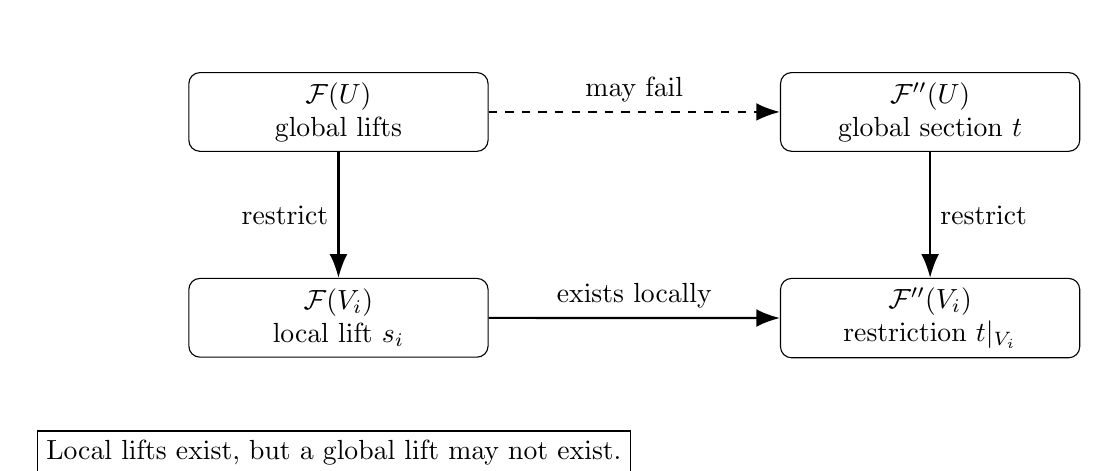
\begin{tikzpicture}[
		node distance=1.6cm,
		box/.style={draw, rounded corners, minimum width=3.8cm, minimum height=1cm, align=center},
		arrow/.style={-{Latex[length=3mm]}, thick},
		dashedarrow/.style={-{Latex[length=3mm]}, thick, dashed}
		]
		
		\node[box] (FU) {$\F(U)$\\ global lifts};
		\node[box, right=3.7cm of FU] (FppU) {$\Fpp(U)$\\ global section \(t\)};
		
		\node[box, below=1.6cm of FU] (FVi) {$\F(V_i)$\\ local lift \(s_i\)};
		\node[box, below=1.6cm of FppU] (FppVi) {$\Fpp(V_i)$\\ restriction \(t|_{V_i}\)};
		
		\draw[dashedarrow] (FU) -- node[above] {may fail} (FppU);
		\draw[arrow] (FVi) -- node[above] {exists locally} (FppVi);
		
		\draw[arrow] (FU) -- node[left] {restrict} (FVi);
		\draw[arrow] (FppU) -- node[right] {restrict} (FppVi);
		
		\node[below=0.8cm of FVi, align=center] (caption) {
			\(\boxed{\text{Local lifts exist, but a global lift may not exist.}}\)
		};
		
	\end{tikzpicture}
\end{center}

This is the key reason why
\[
\Gamma(U,-)
\]
is left exact but not necessarily exact.

\subsection{Exact Sheaf Sequence Versus Global Sections}

Suppose we have a short exact sequence of sheaves:
\[
0\to \Fp\to \F\to \Fpp\to 0.
\]

As sheaves, the sequence is exact.

But after applying sections over \(U\), we get only:
\[
0\to \Gamma(U,\Fp)\to \Gamma(U,\F)\to \Gamma(U,\Fpp).
\]

In general, we do not get a final surjection
\[
\Gamma(U,\F)\to \Gamma(U,\Fpp)\to 0.
\]

This contrast can be summarized as:

\[
\begin{array}{c}
	\textbf{Exact as sheaves:}\\[0.2cm]
	0\to \Fp\to \F\to \Fpp\to 0
	\\[0.8cm]
	\textbf{Only left exact on sections:}\\[0.2cm]
	0\to \Gamma(U,\Fp)\to \Gamma(U,\F)\to \Gamma(U,\Fpp)
	\not\to 0.
\end{array}
\]

Therefore:

\[
\boxed{
	\Gamma(U,-)\text{ preserves kernels but not necessarily surjections.}
}
\]

\subsection{Exponential Sequence Diagram}

The standard example is the exponential sequence on the circle:
\[
0\to \underline{\ZZ}
\to \Czero_{\RR}
\xrightarrow{\exp(2\pi i\,\cdot)}
\Czero_{\SSone}
\to 0.
\]

This is exact as a sequence of sheaves.

The reason is:

\[
\ker\left(\exp(2\pi i\,\cdot)\right)=\underline{\ZZ},
\]
and every circle-valued function locally has a continuous argument.

But after taking global sections over \(S^1\), the sequence becomes:
\[
0\to \Gamma(S^1,\underline{\ZZ})
\to \Gamma(S^1,\Czero_{\RR})
\to \Gamma(S^1,\Czero_{\SSone})
\not\to 0.
\]

The identity map
\[
\id_{S^1}:S^1\to S^1
\]
does not have a global continuous argument.

\[
\begin{array}{c|c}
	\textbf{Local statement} & \textbf{Global statement} \\
	\hline
	\text{Every }S^1\text{-valued function has local arguments.}
	&
	\text{Not every }S^1\text{-valued function has a global argument.}
	\\[0.2cm]
	\text{The sheaf map is surjective.}
	&
	\text{The map on global sections is not surjective.}
\end{array}
\]

\subsection{Circle Picture: Local Angles}

The following picture represents local choices of an angle on arcs of the circle.

\begin{center}
	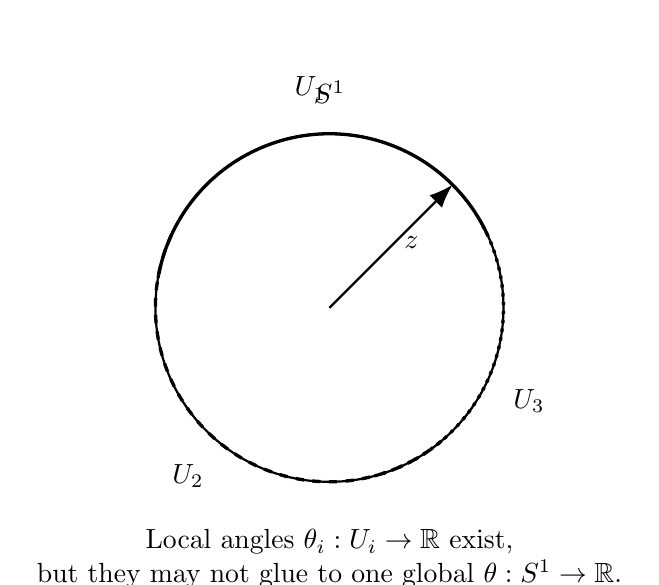
\begin{tikzpicture}[scale=1.3]
		
		\draw[thick] (0,0) circle (1.7);
		
		\draw[very thick] (25:1.7) arc (25:170:1.7);
		\draw[very thick, dashed] (155:1.7) arc (155:310:1.7);
		\draw[very thick, dotted] (285:1.7) arc (285:390:1.7);
		
		\node at (95:2.15) {$U_1$};
		\node at (230:2.15) {$U_2$};
		\node at (335:2.15) {$U_3$};
		
		\node[align=center] at (0,-2.45) {
			Local angles \(\theta_i:U_i\to \RR\) exist,\\
			but they may not glue to one global \(\theta:S^1\to\RR\).
		};
		
		\draw[-{Latex[length=3mm]}, thick] (0,0) -- (45:1.7);
		\node[right] at (45:0.9) {$z$};
		
		\node[above] at (0,1.9) {$S^1$};
		
	\end{tikzpicture}
\end{center}

On overlaps,
\[
e^{2\pi i\theta_i}=e^{2\pi i\theta_j},
\]
so
\[
\theta_i-\theta_j\in \ZZ.
\]

These integer differences on overlaps are the obstruction to gluing the local arguments globally.

\subsection{Skyscraper Sheaf Diagram}

Let \(X=\RR\), fix a point \(p\in X\), and consider the quotient
\[
\Czero_X/\mathcal I_p,
\]
where
\[
\mathcal I_p(U)=
\{f\in \Czero_X(U): f(p)=0 \text{ if }p\in U\}.
\]

Then
\[
\Czero_X/\mathcal I_p\cong \RR_p,
\]
where \(\RR_p\) is the skyscraper sheaf supported at \(p\).

Its stalks are:
\[
(\RR_p)_x=
\begin{cases}
	\RR, & x=p,\\
	0, & x\neq p.
\end{cases}
\]

\begin{center}
	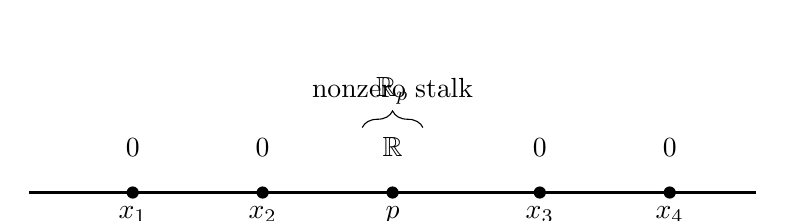
\begin{tikzpicture}[scale=1.1]
		
		\draw[thick] (-4.2,0)--(4.2,0);
		
		\foreach \x/\lab/\val in {-3/$x_1$/$0$, -1.5/$x_2$/$0$, 0/$p$/$\RR$, 1.7/$x_3$/$0$, 3.2/$x_4$/$0$}
		{
			\fill (\x,0) circle (2pt);
			\node[below] at (\x,-0.05) {\lab};
			\node[above] at (\x,0.3) {\val};
		}
		
		\node[above=1cm] at (0,0) {$\RR_p$};
		
		\draw[decorate,decoration={brace,amplitude=6pt}] (-0.35,0.75)--(0.35,0.75);
		\node[above] at (0,0.98) {nonzero stalk};
		
	\end{tikzpicture}
\end{center}

This diagram says that the quotient sheaf has all its information concentrated at one point.

\subsection{Quotient Sheaf Versus Sectionwise Quotient}

For a subsheaf
\[
\Fp\subseteq \F,
\]
one might expect:
\[
(\F/\Fp)(U)=\F(U)/\Fp(U).
\]

But this is not true in general.

The quotient sheaf is:
\[
\F/\Fp=
\left(U\mapsto \F(U)/\Fp(U)\right)^{\#},
\]
the sheafification of the quotient presheaf.

\[
\begin{array}{c|c}
	\textbf{Presheaf quotient} & \textbf{Quotient sheaf} \\
	\hline
	U\mapsto \F(U)/\Fp(U)
	&
	\left(U\mapsto \F(U)/\Fp(U)\right)^{\#}
	\\[0.2cm]
	\text{may fail gluing}
	&
	\text{satisfies locality and gluing}
	\\[0.2cm]
	\text{uses global representatives}
	&
	\text{allows local representatives}
\end{array}
\]

In the exponential example:
\[
\Czero_{\RR}/\underline{\ZZ}
\cong
\Czero_{\SSone}
\]
as sheaves, but
\[
(\Czero_{\RR}/\underline{\ZZ})(S^1)
\neq
\Czero_{\RR}(S^1)/\underline{\ZZ}(S^1).
\]

The identity map
\[
S^1\to S^1
\]
is a global section of the quotient sheaf, but it is not represented by a global real-valued argument.

\[
\boxed{
	\text{Quotient sheaves are local quotients, not necessarily sectionwise quotients.}
}
\]

\subsection{Chart: Three Levels of Exactness}

\[
\begin{array}{>{\raggedright\arraybackslash}p{4cm}
		|>{\raggedright\arraybackslash}p{5cm}
		|>{\raggedright\arraybackslash}p{5cm}}
	\toprule
	\textbf{Level} & \textbf{What it sees} & \textbf{Exactness behavior} \\
	\midrule
	Stalks \(\F_x\)
	&
	Local algebra at one point
	&
	Exactness works like ordinary algebra.
	\\
	\midrule
	Sheaves \(\F\)
	&
	Compatible local data on all open sets
	&
	Exactness is checked stalkwise.
	\\
	\midrule
	Sections \(\Gamma(U,\F)\)
	&
	Global data over \(U\)
	&
	Only left exact in general.
	\\
	\bottomrule
\end{array}
\]

\subsection{Chart: Important Examples}

\[
\begin{array}{>{\raggedright\arraybackslash}p{4.2cm}
		|>{\raggedright\arraybackslash}p{5cm}
		|>{\raggedright\arraybackslash}p{5cm}}
	\toprule
	\textbf{Example} & \textbf{Phenomenon} & \textbf{Main lesson} \\
	\midrule
	\(\Czero_X\xrightarrow{\cdot 2}\Czero_X\)
	&
	Isomorphism of sheaves
	&
	Injective and surjective morphism is an isomorphism.
	\\
	\midrule
	\(\underline{\ZZ}\hookrightarrow \Czero_X\)
	&
	Injective but not surjective
	&
	Subsheaves behave like inclusions.
	\\
	\midrule
	\(\Czero_{\RR}\to \Czero_{\SSone}\)
	&
	Surjective sheaf map, not globally surjective
	&
	Sheaf surjectivity means local liftability.
	\\
	\midrule
	\(0\to \underline{\ZZ}\to \Czero_{\RR}\to \Czero_{\SSone}\to 0\)
	&
	Exponential short exact sequence
	&
	Local logarithms exist, but global logarithms may fail.
	\\
	\midrule
	\(\Czero_X/\mathcal I_p\cong \RR_p\)
	&
	Quotient sheaf is a skyscraper sheaf
	&
	Quotients can concentrate information at a point.
	\\
	\midrule
	\(0\to \mathfrak m_p\to \OO_X\to \CC_p\to 0\)
	&
	Complex-geometric quotient
	&
	A local ring modulo its maximal ideal gives the residue field.
	\\
	\midrule
	\(\Gamma(S^1,-)\) applied to the exponential sequence
	&
	Left exact but not exact
	&
	Global sections do not preserve surjectivity.
	\\
	\bottomrule
\end{array}
\]

\subsection{Final Conceptual Flow Diagram}

\begin{center}
	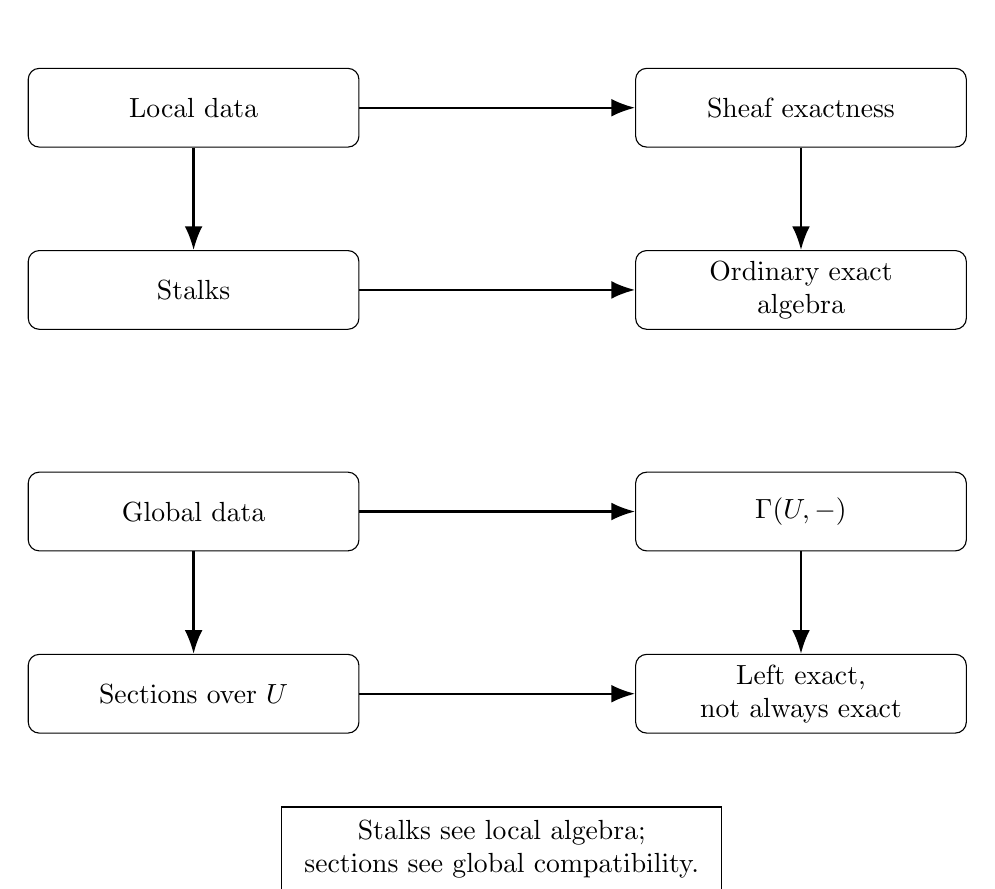
\begin{tikzpicture}[
		node distance=1.5cm,
		box/.style={draw, rounded corners, minimum width=4.2cm, minimum height=1cm, align=center},
		arrow/.style={-{Latex[length=3mm]}, thick}
		]
		
		\node[box] (local) {Local data};
		\node[box, right=3.5cm of local] (sheafexact) {Sheaf exactness};
		
		\node[box, below=1.3cm of local] (stalks) {Stalks};
		\node[box, right=3.5cm of stalks] (algebra) {Ordinary exact\\ algebra};
		
		\node[box, below=1.8cm of stalks] (global) {Global data};
		\node[box, right=3.5cm of global] (gamma) {$\Gamma(U,-)$};
		
		\node[box, below=1.3cm of global] (sections) {Sections over \(U\)};
		\node[box, right=3.5cm of sections] (leftexact) {Left exact,\\ not always exact};
		
		\draw[arrow] (local) -- (sheafexact);
		\draw[arrow] (local) -- (stalks);
		\draw[arrow] (sheafexact) -- (algebra);
		\draw[arrow] (stalks) -- (algebra);
		
		\draw[arrow] (global) -- (gamma);
		\draw[arrow] (global) -- (sections);
		\draw[arrow] (gamma) -- (leftexact);
		\draw[arrow] (sections) -- (leftexact);
		
		% ---- fixed bottom caption (NO \[...\] inside node) ----
		\node[align=center, below=0.8cm of leftexact, xshift=-3.8cm] {$%
			\boxed{\begin{array}{c}
					\text{Stalks see local algebra;}\\
					\text{sections see global compatibility.}
			\end{array}}$};
		
	\end{tikzpicture}
\end{center}


\subsection{Final Summary}

The diagrams show the main structure:

\[
\boxed{
	\text{Sheaf exactness is local.}
}
\]

\[
\boxed{
	\text{Quotient sheaves are locally ordinary quotients.}
}
\]

\[
\boxed{
	\Gamma(U,-)\text{ is left exact but not generally exact.}
}
\]

The essential geometric idea is:

\[
\boxed{
	\text{Local solutions may exist even when global solutions do not.}
}
\]

This is the reason sheaf cohomology appears: it measures the obstruction to gluing local data into global data.


\section{When Injective and Surjective Does Not Imply Isomorphism}

For morphisms of sheaves, the following statement is true:

\[
\varphi:\mathcal F\to \mathcal G
\text{ is an isomorphism}
\quad\Longleftrightarrow\quad
\varphi
\text{ is injective and surjective}.
\]

However, this statement is not true in every category. The reason is that the words
``injective'' and ``surjective'' depend on the category we are working in.

In many algebraic categories, such as sets, groups, rings, and modules, a bijective homomorphism is an isomorphism. But in other categories, a morphism can be both injective and surjective on the underlying sets and still fail to be an isomorphism.

There is also a second related phenomenon: in category theory, one often replaces ``injective'' by \emph{monomorphism} and ``surjective'' by \emph{epimorphism}. A morphism can be both a monomorphism and an epimorphism without being an isomorphism.

\subsection{Counterexample 1: A continuous bijection which is not a homeomorphism}

Consider the category \(\mathbf{Top}\) of topological spaces.

Let
\[
X=\mathbb R_{\mathrm{disc}}
\]
be the set \(\mathbb R\) with the discrete topology, and let
\[
Y=\mathbb R_{\mathrm{usual}}
\]
be the set \(\mathbb R\) with its usual topology.

Consider the identity map on the underlying set:
\[
f:X\to Y,
\qquad
f(x)=x.
\]

This map is bijective as a function:
\[
f \text{ is injective and surjective}.
\]

It is also continuous. Indeed, every subset of \(X=\mathbb R_{\mathrm{disc}}\) is open, so for every open set \(U\subseteq Y\), the preimage
\[
f^{-1}(U)=U
\]
is open in \(X\).

Thus \(f\) is a continuous bijection.

However, \(f\) is not an isomorphism in \(\mathbf{Top}\), because an isomorphism in \(\mathbf{Top}\) is a homeomorphism. The inverse map
\[
f^{-1}:Y\to X
\]
is again the identity function on the underlying set, but it is not continuous.

Indeed, take a subset such as
\[
\{0\}\subseteq X.
\]
This set is open in the discrete topology. But
\[
(f^{-1})^{-1}(\{0\})=\{0\}
\]
is not open in the usual topology on \(\mathbb R\).

Therefore the inverse map is not continuous.

Hence
\[
f:\mathbb R_{\mathrm{disc}}\to \mathbb R_{\mathrm{usual}}
\]
is injective and surjective as a function, but it is not an isomorphism in \(\mathbf{Top}\).

\[
\boxed{
	\text{In } \mathbf{Top},\text{ a continuous bijection need not be an isomorphism.}
}
\]

\subsection{Counterexample 2: The half-open interval mapped to the circle}

Another classical example in \(\mathbf{Top}\) is the map
\[
f:[0,2\pi)\to S^1
\]
defined by
\[
f(t)=e^{it}.
\]

This map is continuous and bijective.

Indeed, every point of the unit circle has a unique argument
\[
t\in [0,2\pi).
\]

So \(f\) is injective and surjective as a function.

However, \(f\) is not a homeomorphism. The inverse map
\[
f^{-1}:S^1\to [0,2\pi)
\]
is not continuous at the point \(1\in S^1\).

Geometrically, when points on the circle approach \(1\) from one side, their arguments approach \(0\), but from the other side their arguments approach \(2\pi\). Thus the inverse has a jump discontinuity.

Therefore
\[
[0,2\pi)\to S^1,
\qquad
t\mapsto e^{it},
\]
is a continuous bijection but not an isomorphism in \(\mathbf{Top}\).

\subsection{Counterexample 3: A monomorphism and epimorphism which is not an isomorphism}

Now we give a categorical example.

In category theory, one says that a morphism
\[
f:A\to B
\]
is a \emph{monomorphism} if it is left-cancellative, meaning that for all objects \(T\) and all morphisms
\[
g,h:T\to A,
\]
we have
\[
f\circ g=f\circ h
\quad\Longrightarrow\quad
g=h.
\]

Similarly, \(f\) is an \emph{epimorphism} if it is right-cancellative, meaning that for all objects \(T\) and all morphisms
\[
g,h:B\to T,
\]
we have
\[
g\circ f=h\circ f
\quad\Longrightarrow\quad
g=h.
\]

In the category of sets, monomorphisms are exactly injective maps, and epimorphisms are exactly surjective maps. But this is not true in every category.

Consider the category \(\mathbf{CRing}\) of commutative rings with identity. The inclusion
\[
\iota:\mathbb Z\hookrightarrow \mathbb Q
\]
is a ring homomorphism.

It is injective as a function, so it is a monomorphism in \(\mathbf{CRing}\).

It is also an epimorphism in \(\mathbf{CRing}\). To see this, suppose \(R\) is a commutative ring and
\[
g,h:\mathbb Q\to R
\]
are ring homomorphisms such that
\[
g\circ \iota=h\circ \iota.
\]
This means that \(g\) and \(h\) agree on \(\mathbb Z\).

But every rational number has the form
\[
\frac{a}{b},
\qquad
a,b\in \mathbb Z,\quad b\neq 0.
\]
If a ring homomorphism \(\mathbb Q\to R\) exists, then it must send
\[
\frac{a}{b}
\]
to
\[
g(a)\,g(b)^{-1}.
\]
Therefore the values of \(g\) and \(h\) on \(\mathbb Z\) determine their values on all of \(\mathbb Q\). Hence
\[
g=h.
\]

So
\[
\iota:\mathbb Z\hookrightarrow \mathbb Q
\]
is both a monomorphism and an epimorphism in \(\mathbf{CRing}\).

However, it is not an isomorphism, because it is not surjective as a function. For example,
\[
\frac{1}{2}\in \mathbb Q
\]
is not in the image of \(\mathbb Z\).

Thus
\[
\mathbb Z\hookrightarrow \mathbb Q
\]
is a monomorphism and an epimorphism, but not an isomorphism.

\[
\boxed{
	\text{In } \mathbf{CRing},\text{ mono + epi does not imply isomorphism.}
}
\]

\subsection{Comparison with sheaves}

For sheaves, the situation is better.

Let
\[
\varphi:\mathcal F\to \mathcal G
\]
be a morphism of sheaves on a topological space \(X\).

Then
\[
\varphi
\text{ is an isomorphism}
\]
if and only if for every point \(x\in X\), the induced map on stalks
\[
\varphi_x:\mathcal F_x\to \mathcal G_x
\]
is an isomorphism.

Therefore, if \(\varphi\) is injective and surjective as a morphism of sheaves, then each stalk map
\[
\varphi_x:\mathcal F_x\to \mathcal G_x
\]
is both injective and surjective. Hence it is bijective, and therefore an isomorphism.

It follows that
\[
\varphi:\mathcal F\to \mathcal G
\]
is an isomorphism of sheaves.

Thus:

\[
\boxed{
	\text{For sheaves, injective + surjective implies isomorphism.}
}
\]

\subsection{Summary table}

\[
\begin{array}{c|c|c|c}
	\textbf{Category}
	&
	\textbf{Morphism}
	&
	\textbf{Injective/Surjective?}
	&
	\textbf{Isomorphism?}
	\\
	\hline
	\mathbf{Set}
	&
	\text{bijective function}
	&
	\text{yes}
	&
	\text{yes}
	\\[4pt]
	\mathbf{Grp}
	&
	\text{bijective group homomorphism}
	&
	\text{yes}
	&
	\text{yes}
	\\[4pt]
	\mathbf{Mod}_R
	&
	\text{bijective module homomorphism}
	&
	\text{yes}
	&
	\text{yes}
	\\[4pt]
	\mathbf{Top}
	&
	\mathbb R_{\mathrm{disc}}\to \mathbb R_{\mathrm{usual}}
	&
	\text{yes}
	&
	\text{no}
	\\[4pt]
	\mathbf{Top}
	&
	[0,2\pi)\to S^1
	&
	\text{yes}
	&
	\text{no}
	\\[4pt]
	\mathbf{CRing}
	&
	\mathbb Z\hookrightarrow \mathbb Q
	&
	\text{mono and epi}
	&
	\text{no}
	\\[4pt]
	\mathbf{Sh}(X)
	&
	\mathcal F\to \mathcal G
	&
	\text{injective and surjective}
	&
	\text{yes}
\end{array}
\]

\subsection{Main conclusion}

The statement

\[
\text{injective + surjective}
\quad\Longrightarrow\quad
\text{isomorphism}
\]

is true for sheaves, sets, groups, rings, and modules when injective and surjective are understood on the correct underlying algebraic objects.

However, it fails in categories where an isomorphism requires extra structure to be preserved by the inverse.

The most important example is the category of topological spaces:

\[
\boxed{
	\text{A continuous bijection need not be a homeomorphism.}
}
\]

Categorically, an even subtler failure is:

\[
\boxed{
	\text{A morphism can be both monic and epic without being an isomorphism.}
}
\]

For example,

\[
\boxed{
	\mathbb Z\hookrightarrow \mathbb Q
}
\]

is both a monomorphism and an epimorphism in \(\mathbf{CRing}\), but it is not an isomorphism.

\subsection{The morphism \texorpdfstring{\(\mathbb Z\to \mathbb C\)}{Z to C}}

Consider the unital ring homomorphism
\[
\iota:\mathbb Z\longrightarrow \mathbb C
\]
defined by
\[
\iota(n)=n\cdot 1_{\mathbb C}.
\]

This is the standard inclusion of the integers into the complex numbers:
\[
\mathbb Z\subseteq \mathbb C.
\]

\subsubsection*{It is injective}

The map is injective because different integers define different complex numbers. Equivalently,
\[
\ker(\iota)=0.
\]

Therefore \(\iota\) is a monomorphism in the category of commutative rings.

\subsubsection*{It is not surjective}

The map is not surjective as a function because most complex numbers are not integers. For example,
\[
i\in \mathbb C
\]
is not in the image of \(\mathbb Z\).

Also,
\[
\frac{1}{2}\in \mathbb C
\]
is not in the image of \(\mathbb Z\).

Therefore
\[
\mathbb Z\to \mathbb C
\]
is not an isomorphism of rings.

\subsubsection*{It is not an epimorphism in \(\mathbf{CRing}\)}

Unlike the map
\[
\mathbb Z\hookrightarrow \mathbb Q,
\]
the map
\[
\mathbb Z\hookrightarrow \mathbb C
\]
is not an epimorphism in the category of commutative rings.

To see this, consider two ring homomorphisms
\[
g,h:\mathbb C\to \mathbb C.
\]

Let
\[
g=\operatorname{id}_{\mathbb C}
\]
be the identity map, and let
\[
h:\mathbb C\to \mathbb C
\]
be complex conjugation:
\[
h(z)=\overline z.
\]

Both \(g\) and \(h\) are unital ring homomorphisms.

They agree on \(\mathbb Z\), because for every integer \(n\),
\[
g(n)=n
\]
and
\[
h(n)=\overline n=n.
\]

Thus
\[
g\circ \iota=h\circ \iota.
\]

However,
\[
g\neq h,
\]
because
\[
g(i)=i,
\qquad
h(i)=\overline i=-i.
\]

Therefore there exist two different morphisms
\[
g,h:\mathbb C\to \mathbb C
\]
which become equal after composition with
\[
\iota:\mathbb Z\to \mathbb C.
\]

Hence \(\iota\) is not an epimorphism in \(\mathbf{CRing}\).

\[
\boxed{
	\mathbb Z\to \mathbb C
	\text{ is monic but not epic, and therefore not an isomorphism.}
}
\]

\subsubsection*{Comparison with \(\mathbb Z\to \mathbb Q\)}

The map
\[
\mathbb Z\hookrightarrow \mathbb Q
\]
is different.

It is not surjective as a function, but it is an epimorphism in \(\mathbf{CRing}\). The reason is that any ring homomorphism out of \(\mathbb Q\) is determined by its values on \(\mathbb Z\), because every rational number has the form
\[
\frac{a}{b},
\qquad a,b\in\mathbb Z,\quad b\neq 0.
\]

So if two ring maps
\[
g,h:\mathbb Q\to R
\]
agree on \(\mathbb Z\), then they must agree on all fractions:
\[
g\left(\frac{a}{b}\right)
=
g(a)g(b)^{-1},
\]
and similarly for \(h\).

Therefore
\[
\mathbb Z\to \mathbb Q
\]
is an epimorphism in \(\mathbf{CRing}\).

But
\[
\mathbb Z\to \mathbb C
\]
is not an epimorphism, because \(\mathbb C\) has nontrivial automorphisms over \(\mathbb Z\), for example complex conjugation.

\subsubsection*{Geometric interpretation}

The ring morphism
\[
\mathbb Z\to \mathbb C
\]
induces a morphism of affine schemes in the opposite direction:
\[
\operatorname{Spec}\mathbb C\longrightarrow \operatorname{Spec}\mathbb Z.
\]

Since \(\mathbb C\) is a field,
\[
\operatorname{Spec}\mathbb C
\]
has exactly one point, namely
\[
(0).
\]

The image of this point under
\[
\operatorname{Spec}\mathbb C\to \operatorname{Spec}\mathbb Z
\]
is the inverse image of the prime ideal \((0)\subseteq \mathbb C\):
\[
\iota^{-1}((0))=(0)\subseteq \mathbb Z.
\]

Thus the unique point of \(\operatorname{Spec}\mathbb C\) maps to the generic point of
\[
\operatorname{Spec}\mathbb Z.
\]

So geometrically,
\[
\operatorname{Spec}\mathbb C\to \operatorname{Spec}\mathbb Z
\]
is a point lying over the generic point of \(\operatorname{Spec}\mathbb Z\), not over a closed prime \((p)\).

\[
\boxed{
	\operatorname{Spec}\mathbb C\to \operatorname{Spec}\mathbb Z
	\text{ maps the unique point of }\operatorname{Spec}\mathbb C
	\text{ to the generic point }(0)\in\operatorname{Spec}\mathbb Z.
}
\]
\section{The Morphisms \texorpdfstring{\(\mathbb Z\to \mathbb C\)}{Z to C}
	and \texorpdfstring{\(\mathbb Z\to \mathbb Q\)}{Z to Q}}

We now explain the scheme-theoretic meaning of the ring morphisms
\[
\mathbb Z\longrightarrow \mathbb C
\]
and
\[
\mathbb Z\longrightarrow \mathbb Q.
\]

The key point is that a ring morphism
\[
\varphi:A\to B
\]
induces a morphism of affine schemes in the opposite direction:
\[
\Spec B\longrightarrow \Spec A.
\]

On points, this map sends a prime ideal
\[
\mathfrak q\subseteq B
\]
to its inverse image, or contraction,
\[
\varphi^{-1}(\mathfrak q)\subseteq A.
\]

Thus the map on prime spectra is
\[
\Spec B\to \Spec A,
\qquad
\mathfrak q\mapsto \varphi^{-1}(\mathfrak q).
\]

\subsection{Prime ideals of \texorpdfstring{\(\mathbb Z\)}{Z}}

Recall that
\[
\Spec \mathbb Z
\]
consists of the prime ideals of \(\mathbb Z\).

These are:
\[
(0)
\]
and
\[
(p)
\]
for every prime number \(p\).

Thus we may write
\[
\Spec \mathbb Z
=
\{(0)\}\cup \{(p):p\text{ prime}\}.
\]

The point \((0)\) is the generic point of \(\Spec\mathbb Z\), because
\[
\overline{\{(0)\}}=\Spec\mathbb Z.
\]

The points \((p)\) are closed points. Indeed, the quotient
\[
\mathbb Z/(p)
\]
is the finite field
\[
\mathbb F_p,
\]
so \((p)\) is a maximal ideal of \(\mathbb Z\).

Thus the picture is:

\[
\begin{array}{c}
	\eta=(0)\quad \text{generic point}
	\\[6pt]
	\downarrow
	\\[6pt]
	(p)\quad \text{closed points, one for each prime }p
\end{array}
\]

Geometrically, \(\Spec\mathbb Z\) behaves like an arithmetic curve. The generic point corresponds to characteristic \(0\), while the closed point \((p)\) corresponds to characteristic \(p\).

\subsection{The morphism \texorpdfstring{\(\mathbb Z\to \mathbb C\)}{Z to C}}

Consider the natural ring homomorphism
\[
\iota:\mathbb Z\longrightarrow \mathbb C
\]
defined by
\[
\iota(n)=n\cdot 1_{\mathbb C}.
\]

This is the usual inclusion of the integers into the complex numbers.

Since \(\mathbb C\) is a field, it has only two ideals:
\[
(0)
\qquad\text{and}\qquad
\mathbb C.
\]
The only prime ideal is
\[
(0).
\]

Therefore
\[
\Spec\mathbb C
\]
has exactly one point:
\[
\Spec\mathbb C=\{(0)\}.
\]

The ring morphism
\[
\mathbb Z\to \mathbb C
\]
induces a scheme morphism
\[
\Spec\mathbb C\longrightarrow \Spec\mathbb Z.
\]

To determine where the unique point of \(\Spec\mathbb C\) goes, we take the inverse image of the prime ideal
\[
(0)\subseteq \mathbb C.
\]

We compute:
\[
\iota^{-1}((0))
=
\{n\in \mathbb Z:\iota(n)=0\in \mathbb C\}.
\]

But \(\mathbb C\) has characteristic \(0\). Hence
\[
n\cdot 1_{\mathbb C}=0
\]
if and only if
\[
n=0.
\]

Therefore
\[
\iota^{-1}((0))=(0)\subseteq \mathbb Z.
\]

So the unique point of \(\Spec\mathbb C\) maps to the generic point of \(\Spec\mathbb Z\):

\[
\begin{array}{ccc}
	\Spec\mathbb C & \longrightarrow & \Spec\mathbb Z
	\\[6pt]
	(0) & \longmapsto & (0).
\end{array}
\]

Thus
\[
\boxed{
	\Spec\mathbb C\to \Spec\mathbb Z
	\text{ lands at the generic point of }\Spec\mathbb Z.
}
\]

\subsection{Why it does not land over a closed point}

A closed point of \(\Spec\mathbb Z\) has the form
\[
(p)
\]
for a prime number \(p\).

For the point of \(\Spec\mathbb C\) to map to \((p)\), we would need
\[
\iota^{-1}((0))=(p).
\]

But this would mean that
\[
p\cdot 1_{\mathbb C}=0.
\]

That is false, because \(\mathbb C\) has characteristic \(0\).

In fact, every nonzero integer becomes a nonzero complex number, and therefore no prime number \(p\) becomes zero in \(\mathbb C\).

Thus the morphism
\[
\Spec\mathbb C\to \Spec\mathbb Z
\]
does not land over any closed point \((p)\). It lands over the generic point \((0)\).

\subsection{Residue field interpretation for \texorpdfstring{\(\mathbb Z\to \mathbb C\)}{Z to C}}

The residue field at the generic point
\[
(0)\in \Spec\mathbb Z
\]
is
\[
\kappa((0))=\operatorname{Frac}(\mathbb Z)=\mathbb Q.
\]

The morphism
\[
\Spec\mathbb C\to \Spec\mathbb Z
\]
therefore gives a field extension at the generic point:
\[
\kappa((0))=\mathbb Q
\longrightarrow
\mathbb C.
\]

So scheme-theoretically, the morphism
\[
\Spec\mathbb C\to \Spec\mathbb Z
\]
is a point lying over the generic point of \(\Spec\mathbb Z\), together with an extension of residue fields
\[
\mathbb Q\subseteq \mathbb C.
\]

Thus one may think of \(\Spec\mathbb C\) as a geometric point over the generic point of \(\Spec\mathbb Z\).

\subsection{The morphism \texorpdfstring{\(\mathbb Z\to \mathbb Q\)}{Z to Q}}

Now consider the natural inclusion
\[
j:\mathbb Z\longrightarrow \mathbb Q.
\]

Again, since \(\mathbb Q\) is a field, the scheme
\[
\Spec\mathbb Q
\]
has exactly one point:
\[
\Spec\mathbb Q=\{(0)\}.
\]

The ring morphism
\[
\mathbb Z\to \mathbb Q
\]
induces a scheme morphism
\[
\Spec\mathbb Q\longrightarrow \Spec\mathbb Z.
\]

The unique point \((0)\in \Spec\mathbb Q\) maps to
\[
j^{-1}((0))\subseteq \mathbb Z.
\]

We compute:
\[
j^{-1}((0))
=
\{n\in\mathbb Z:j(n)=0\in\mathbb Q\}.
\]

But the inclusion
\[
\mathbb Z\hookrightarrow \mathbb Q
\]
is injective, so
\[
j(n)=0
\]
if and only if
\[
n=0.
\]

Hence
\[
j^{-1}((0))=(0).
\]

Therefore
\[
\begin{array}{ccc}
	\Spec\mathbb Q & \longrightarrow & \Spec\mathbb Z
	\\[6pt]
	(0) & \longmapsto & (0).
\end{array}
\]

So
\[
\boxed{
	\Spec\mathbb Q\to \Spec\mathbb Z
	\text{ also lands at the generic point of }\Spec\mathbb Z.
}
\]

\subsection{Localization viewpoint for \texorpdfstring{\(\mathbb Z\to \mathbb Q\)}{Z to Q}}

The map
\[
\mathbb Z\to \mathbb Q
\]
is the localization of \(\mathbb Z\) at all nonzero integers.

Let
\[
S=\mathbb Z\setminus\{0\}.
\]
Then
\[
\mathbb Q=S^{-1}\mathbb Z.
\]

For a localization
\[
A\to S^{-1}A,
\]
the induced morphism
\[
\Spec S^{-1}A\to \Spec A
\]
identifies \(\Spec S^{-1}A\) with the set of prime ideals of \(A\) which do not meet \(S\).

In our case, \(A=\mathbb Z\) and
\[
S=\mathbb Z\setminus\{0\}.
\]

A prime ideal \(\mathfrak p\subseteq \mathbb Z\) survives in
\[
S^{-1}\mathbb Z=\mathbb Q
\]
if and only if
\[
\mathfrak p\cap S=\varnothing.
\]

Now consider the prime ideals of \(\mathbb Z\):

\[
(0),\quad (2),\quad (3),\quad (5),\quad \dots
\]

The ideal \((0)\) does not meet \(S\), because
\[
(0)\cap(\mathbb Z\setminus\{0\})=\varnothing.
\]

But every nonzero prime ideal \((p)\) does meet \(S\), because
\[
p\in (p)
\]
and
\[
p\in S.
\]

Therefore the only prime ideal of \(\mathbb Z\) that survives after localizing at all nonzero integers is
\[
(0).
\]

Hence
\[
\Spec\mathbb Q
\]
maps to the single point
\[
(0)\in \Spec\mathbb Z.
\]

So the map
\[
\Spec\mathbb Q\to \Spec\mathbb Z
\]
selects precisely the generic point of \(\Spec\mathbb Z\).

\subsection{Comparison between \texorpdfstring{\(\mathbb Z\to \mathbb Q\)}{Z to Q}
	and \texorpdfstring{\(\mathbb Z\to \mathbb C\)}{Z to C}}

Both maps
\[
\mathbb Z\to \mathbb Q
\]
and
\[
\mathbb Z\to \mathbb C
\]
induce morphisms whose unique source point maps to the generic point of
\[
\Spec\mathbb Z.
\]

Thus, topologically, both maps look like
\[
\{\text{one point}\}\longrightarrow \Spec\mathbb Z,
\]
where that one point lands at
\[
(0)\in \Spec\mathbb Z.
\]

However, they differ in the residue field extension.

For
\[
\Spec\mathbb Q\to \Spec\mathbb Z,
\]
the residue field extension over the generic point is
\[
\mathbb Q\to \mathbb Q.
\]

This is the identity extension.

For
\[
\Spec\mathbb C\to \Spec\mathbb Z,
\]
the residue field extension over the generic point is
\[
\mathbb Q\to \mathbb C.
\]

So \(\Spec\mathbb C\) is not just the generic point itself. It is a point over the generic point with a larger residue field.

\[
\begin{array}{c|c|c|c}
	\textbf{Ring map}
	&
	\textbf{Scheme map}
	&
	\textbf{Image in }\Spec\mathbb Z
	&
	\textbf{Residue field extension}
	\\
	\hline
	\mathbb Z\to \mathbb Q
	&
	\Spec\mathbb Q\to \Spec\mathbb Z
	&
	(0)
	&
	\mathbb Q\to \mathbb Q
	\\[5pt]
	\mathbb Z\to \mathbb C
	&
	\Spec\mathbb C\to \Spec\mathbb Z
	&
	(0)
	&
	\mathbb Q\to \mathbb C
\end{array}
\]

\subsection{Comparison with \texorpdfstring{\(\mathbb Z\to \mathbb F_p\)}{Z to Fp}}

To see the contrast, consider the quotient map
\[
\mathbb Z\to \mathbb F_p.
\]

Since
\[
\mathbb F_p=\mathbb Z/(p),
\]
the kernel of this map is
\[
(p).
\]

The induced morphism is
\[
\Spec\mathbb F_p\to \Spec\mathbb Z.
\]

Again, \(\mathbb F_p\) is a field, so
\[
\Spec\mathbb F_p
\]
has one point:
\[
(0).
\]

The image of this point is
\[
\mathbb Z^{-1}((0))=(p).
\]

More explicitly,
\[
\{n\in\mathbb Z:n\equiv 0\pmod p\}=(p).
\]

Therefore
\[
\Spec\mathbb F_p\to \Spec\mathbb Z
\]
lands at the closed point
\[
(p)\in\Spec\mathbb Z.
\]

Thus:

\[
\begin{array}{c|c|c}
	\textbf{Ring map}
	&
	\textbf{Scheme map}
	&
	\textbf{Where the point lands}
	\\
	\hline
	\mathbb Z\to \mathbb Q
	&
	\Spec\mathbb Q\to \Spec\mathbb Z
	&
	(0)\text{, the generic point}
	\\[5pt]
	\mathbb Z\to \mathbb C
	&
	\Spec\mathbb C\to \Spec\mathbb Z
	&
	(0)\text{, the generic point}
	\\[5pt]
	\mathbb Z\to \mathbb F_p
	&
	\Spec\mathbb F_p\to \Spec\mathbb Z
	&
	(p)\text{, a closed point}
\end{array}
\]

\subsection{Geometric summary}

The scheme
\[
\Spec\mathbb Z
\]
has one generic point,
\[
(0),
\]
and closed points
\[
(p)
\]
for every prime number \(p\).

The morphism
\[
\Spec\mathbb Q\to \Spec\mathbb Z
\]
is the generic point itself, with residue field
\[
\mathbb Q.
\]

The morphism
\[
\Spec\mathbb C\to \Spec\mathbb Z
\]
is also a point over the generic point, but with larger residue field
\[
\mathbb C.
\]

The morphism
\[
\Spec\mathbb F_p\to \Spec\mathbb Z
\]
is a point over the closed point
\[
(p).
\]

In short:

\[
\boxed{
	\Spec\mathbb Q
	\text{ and }
	\Spec\mathbb C
	\text{ lie over the generic point of }
	\Spec\mathbb Z.
}
\]

But:

\[
\boxed{
	\Spec\mathbb F_p
	\text{ lies over the closed point }(p).
}
\]


\subsection{Explicit Ring Maps \texorpdfstring{\(\mathbb Z\to \mathbb Q\)}{Z to Q}
	and \texorpdfstring{\(\mathbb Z\to \mathbb C\)}{Z to C}}

We now describe explicitly the two natural ring morphisms
\[
\mathbb Z\longrightarrow \mathbb Q
\qquad\text{and}\qquad
\mathbb Z\longrightarrow \mathbb C.
\]

Both are unital ring homomorphisms, meaning that they send
\[
1_{\mathbb Z}
\]
to the multiplicative identity of the target ring.

\subsubsection*{The ring map \texorpdfstring{\(\mathbb Z\to \mathbb Q\)}{Z to Q}}

The natural morphism
\[
j:\mathbb Z\longrightarrow \mathbb Q
\]
is defined by
\[
j(n)=\frac{n}{1}.
\]

Thus
\[
0\mapsto 0,
\qquad
1\mapsto 1,
\qquad
2\mapsto 2,
\qquad
-3\mapsto -3,
\]
and so on.

Equivalently, this is the usual inclusion
\[
\mathbb Z\subseteq \mathbb Q.
\]

It is a ring homomorphism because for all \(m,n\in\mathbb Z\),
\[
j(m+n)=\frac{m+n}{1}
=
\frac{m}{1}+\frac{n}{1}
=
j(m)+j(n),
\]
and
\[
j(mn)=\frac{mn}{1}
=
\frac{m}{1}\cdot \frac{n}{1}
=
j(m)j(n).
\]

Also,
\[
j(1)=1.
\]

The kernel is
\[
\ker(j)=\{n\in\mathbb Z:j(n)=0\in\mathbb Q\}.
\]

But
\[
\frac{n}{1}=0
\]
in \(\mathbb Q\) if and only if
\[
n=0.
\]

Hence
\[
\ker(j)=(0).
\]

Therefore
\[
j:\mathbb Z\to\mathbb Q
\]
is injective.

However, it is not surjective as a function, because for example
\[
\frac12\in\mathbb Q
\]
is not in the image of \(\mathbb Z\).

\subsubsection*{The induced scheme morphism for \texorpdfstring{\(\mathbb Z\to\mathbb Q\)}{Z to Q}}

The ring map
\[
j:\mathbb Z\to\mathbb Q
\]
induces a morphism of affine schemes in the opposite direction:
\[
\Spec\mathbb Q\longrightarrow \Spec\mathbb Z.
\]

Since \(\mathbb Q\) is a field,
\[
\Spec\mathbb Q=\{(0)\}.
\]

The unique point \((0)\in\Spec\mathbb Q\) maps to its contraction:
\[
j^{-1}((0))\subseteq \mathbb Z.
\]

But
\[
j^{-1}((0))=\ker(j)=(0).
\]

Therefore
\[
\begin{array}{ccc}
	\Spec\mathbb Q & \longrightarrow & \Spec\mathbb Z
	\\[4pt]
	(0) & \longmapsto & (0).
\end{array}
\]

Thus \(\Spec\mathbb Q\) maps to the generic point of \(\Spec\mathbb Z\).

The residue field at the generic point of \(\Spec\mathbb Z\) is
\[
\kappa((0))=\operatorname{Frac}(\mathbb Z)=\mathbb Q.
\]

The residue field of the unique point of \(\Spec\mathbb Q\) is
\[
\kappa((0))=\mathbb Q.
\]

Hence the induced residue field map is
\[
\mathbb Q\longrightarrow \mathbb Q,
\]
which is the identity map.

So the morphism
\[
\Spec\mathbb Q\to \Spec\mathbb Z
\]
is the generic point of \(\Spec\mathbb Z\) with residue field \(\mathbb Q\).

\subsubsection*{The localization interpretation of \texorpdfstring{\(\mathbb Z\to\mathbb Q\)}{Z to Q}}

The map
\[
\mathbb Z\to\mathbb Q
\]
is the localization of \(\mathbb Z\) at all nonzero integers.

Let
\[
S=\mathbb Z\setminus\{0\}.
\]

Then
\[
\mathbb Q=S^{-1}\mathbb Z.
\]

So
\[
\mathbb Z\to\mathbb Q
\]
is explicitly
\[
n\longmapsto \frac{n}{1}.
\]

The prime ideals of \(\mathbb Z\) are
\[
(0)
\qquad\text{and}\qquad
(p)
\]
for prime numbers \(p\).

Under localization at \(S\), only those prime ideals disjoint from \(S\) survive.

Now
\[
(0)\cap S=\varnothing,
\]
but for every prime \(p\),
\[
(p)\cap S\neq\varnothing,
\]
because
\[
p\in(p)
\qquad\text{and}\qquad
p\in S.
\]

Therefore only the prime ideal
\[
(0)
\]
survives after localizing \(\mathbb Z\) to \(\mathbb Q\).

This is why
\[
\Spec\mathbb Q\to\Spec\mathbb Z
\]
has image exactly the generic point \((0)\).

\subsubsection*{The ring map \texorpdfstring{\(\mathbb Z\to \mathbb C\)}{Z to C}}

Now consider the natural morphism
\[
\iota:\mathbb Z\longrightarrow \mathbb C.
\]

It is defined by
\[
\iota(n)=n\cdot 1_{\mathbb C}.
\]

Equivalently,
\[
\iota(n)=n+0i.
\]

Thus
\[
0\mapsto 0,
\qquad
1\mapsto 1,
\qquad
2\mapsto 2,
\qquad
-3\mapsto -3,
\]
viewing each integer as a complex number.

Again, \(\iota\) is a ring homomorphism because for all \(m,n\in\mathbb Z\),
\[
\iota(m+n)=(m+n)+0i
=
(m+0i)+(n+0i)
=
\iota(m)+\iota(n),
\]
and
\[
\iota(mn)=mn+0i
=
(m+0i)(n+0i)
=
\iota(m)\iota(n).
\]

Also,
\[
\iota(1)=1_{\mathbb C}.
\]

The kernel is
\[
\ker(\iota)=\{n\in\mathbb Z:\iota(n)=0\in\mathbb C\}.
\]

But
\[
n+0i=0
\]
if and only if
\[
n=0.
\]

Therefore
\[
\ker(\iota)=(0).
\]

So
\[
\iota:\mathbb Z\to\mathbb C
\]
is injective.

It is not surjective as a function, because for example
\[
i\in\mathbb C
\]
is not in the image of \(\mathbb Z\). Also,
\[
\frac12\in\mathbb C
\]
is not in the image of \(\mathbb Z\).

\subsubsection*{The induced scheme morphism for \texorpdfstring{\(\mathbb Z\to\mathbb C\)}{Z to C}}

The ring morphism
\[
\iota:\mathbb Z\to\mathbb C
\]
induces a morphism of affine schemes
\[
\Spec\mathbb C\longrightarrow \Spec\mathbb Z.
\]

Since \(\mathbb C\) is a field,
\[
\Spec\mathbb C=\{(0)\}.
\]

The unique point \((0)\in\Spec\mathbb C\) maps to the contraction
\[
\iota^{-1}((0))\subseteq\mathbb Z.
\]

But
\[
\iota^{-1}((0))=\ker(\iota)=(0).
\]

Therefore
\[
\begin{array}{ccc}
	\Spec\mathbb C & \longrightarrow & \Spec\mathbb Z
	\\[4pt]
	(0) & \longmapsto & (0).
\end{array}
\]

Thus \(\Spec\mathbb C\) also maps to the generic point of \(\Spec\mathbb Z\).

The residue field at the generic point of \(\Spec\mathbb Z\) is
\[
\kappa((0))=\mathbb Q.
\]

The residue field of the unique point of \(\Spec\mathbb C\) is
\[
\kappa((0))=\mathbb C.
\]

Therefore the induced residue field map is
\[
\mathbb Q\longrightarrow \mathbb C.
\]

This is the usual inclusion
\[
\frac{a}{b}\longmapsto \frac{a}{b}+0i.
\]

So the morphism
\[
\Spec\mathbb C\to\Spec\mathbb Z
\]
is a point lying over the generic point of \(\Spec\mathbb Z\), but with residue field \(\mathbb C\), not merely \(\mathbb Q\).

\subsubsection*{Comparison of the two explicit maps}

\[
\begin{array}{c|c|c}
	\textbf{Map}
	&
	\textbf{Formula}
	&
	\textbf{Kernel}
	\\
	\hline
	j:\mathbb Z\to\mathbb Q
	&
	j(n)=\dfrac{n}{1}
	&
	(0)
	\\[10pt]
	\iota:\mathbb Z\to\mathbb C
	&
	\iota(n)=n+0i
	&
	(0)
\end{array}
\]

Both maps are injective.

Neither map is surjective as a function:
\[
\frac12\in\mathbb Q
\]
is not in the image of \(\mathbb Z\), and
\[
i\in\mathbb C
\]
is not in the image of \(\mathbb Z\).

Both induced scheme morphisms send the unique point of the source to the generic point of \(\Spec\mathbb Z\):

\[
\begin{array}{c|c|c}
	\textbf{Ring map}
	&
	\textbf{Scheme map}
	&
	\textbf{Image point in }\Spec\mathbb Z
	\\
	\hline
	\mathbb Z\to\mathbb Q
	&
	\Spec\mathbb Q\to\Spec\mathbb Z
	&
	(0)
	\\[5pt]
	\mathbb Z\to\mathbb C
	&
	\Spec\mathbb C\to\Spec\mathbb Z
	&
	(0)
\end{array}
\]

But their residue field extensions are different:

\[
\begin{array}{c|c}
	\textbf{Scheme morphism}
	&
	\textbf{Residue field extension over }(0)
	\\
	\hline
	\Spec\mathbb Q\to\Spec\mathbb Z
	&
	\mathbb Q\to\mathbb Q
	\\[5pt]
	\Spec\mathbb C\to\Spec\mathbb Z
	&
	\mathbb Q\to\mathbb C
\end{array}
\]

Therefore:
\[
\boxed{
	\Spec\mathbb Q
	\text{ is the generic point of }
	\Spec\mathbb Z
	\text{ with residue field }\mathbb Q.
}
\]

Whereas:
\[
\boxed{
	\Spec\mathbb C
	\text{ is a point over the generic point of }
	\Spec\mathbb Z
	\text{ with larger residue field }\mathbb C.
}
\]

\end{document}